%\documentclass{elsart}       %% one column for review, preprint
\documentclass{elsart3p}    %% two columns for publication
\usepackage{graphicx,amssymb}
\usepackage{times}
\usepackage{helvet}
\usepackage{courier}
\usepackage{url}
\usepackage{latexsym}
\usepackage{verbatim}
\usepackage{xspace}
\usepackage{algorithm}
\usepackage{float}
\usepackage{multirow} 
\usepackage{bigstrut}
%\usepackage{algorithmic}

\usepackage{amstext} % for text in math forumla
\usepackage{indentfirst} % make the first paragraph also indent

\renewcommand\floatpagefraction{.2}
\makeatletter
\def\elsartstyle{%
    \def\normalsize{\@setfontsize\normalsize\@xiipt{14.5}}
    \def\small{\@setfontsize\small\@xipt{13.6}}
    \let\footnotesize=\small
    \def\large{\@setfontsize\large\@xivpt{18}}
    \def\Large{\@setfontsize\Large\@xviipt{22}}
    \skip\@mpfootins = 18\p@ \@plus 2\p@
    \normalsize
}
\@ifundefined{square}{}{\let\Box\square}
\makeatother


\newtheorem{definition}{Definition}
\newtheorem{example}{Example}
\newtheorem{proposition}{Proposition}
\newcommand{\dtr}[1]{(\textbf{Thanh: #1})}

\long\def\symbolfootnote[#1]#2{\begingroup%
\def\thefootnote{\fnsymbol{footnote}}\footnote[#1]{#2}\endgroup}
%\renewcommand{\baselinestretch}{0.965}


\begin{document}
\begin{frontmatter}

% first the title is needed
\title{Semantic Search -- A Unified View of Data and Document Retrieval}

%\author{Thanh Tran\corauthref{C}},
%\ead{duc.tran@kit.de}
%\author{Daniel Herzig},
%\ead{duc.tran@kit.de}

%% these specify any 'notes' for the title and authors,
%% including 'thanks' that acknowledge support, etc. and an
%% indication of who the corresponding author is if there's
%% more than one author.

\corauth[C]{Corresponding author. Tel: +49 (721) 608 4754 }

\medskip

%% Here are the addresses refereenced for the authors.  If
%% all of the authors are from the same institution you need
%% not have the lables for the author and address commands.
%\address{Institute AIFB, Karlsruhe Institute of Technology, D-76128 Karlsruhe, Germany}


\begin{abstract}
\end{abstract}


\begin{keyword}
Search, semantic Search, data retrieval, semantic data retrieval
\end{keyword}
\end{frontmatter}


\section{Introduction}
% unsolved information needs%
Advancements in search technologies enable users to deal and to exploit the ever increasing amount of information that we can find in different scenarios -- from the personal desktop to enterprises' databases up to the large-scale Web. As opposed to the structured querying capabilities commonly provided by commercial databases that are only accessible by experts, \emph{search} is rather understood as a \emph{end-user oriented paradigm} that is based on \emph{intuitive interfaces} and access mechanisms. Solutions that are widely used especially on the Web are based on \emph{keyword search}, and in smaller-scale scenarios, also support natural language (NL) inputs. While they are easy to use, the inputs provided by the users through these interfaces are \emph{ambiguous} such that the underlying information need (query intent) is not directly accessible to the system. Further, there are search scenarios where not only the query, but also the data representation does not precisely capture the semantics and structure of the underlying information. Accordingly, the core problems to be addressed in search are to \emph{understand the query intent and the data}, to \emph{match query against data}, and to \emph{rank results}. 

\subsection{Many Unsolved Long-tail Queries}
Modern search engines can effectively interpret the topics and based on that, disambiguates the need intended in the provided query inputs. Combining with additional (query-independent) factors such as PageRank, they are able to address a large fraction fraction of common information needs. In particular, queries that request for pages about a particular topic (\emph{topical query}) or representing popular entry points to commonly used information that can be reached via further browsing activities (\emph{navigational queries}), can be successfully processed. However, dealing with the large number of distinct queries in the ``long tail'' of Web query logs \cite{} remains challenging. Two particular categories of problematic cases are ambiguous and complex queries:

\begin{itemize}
	\item \emph{Ambiguous queries}: these queries contain ambiguous terms, resulting in many possible interpretations (several query intents). For instance, the query ``young scholars from Germany'' is difficult to processed because without any additional context, it is not clear who is ``young'', and different types of people may be considered as ``scholars''. 

	\item \emph{Complex queries}: this class of queries capture complex information needs which may involve several entities and relationships between them. As an example, we have a query that mentions a person and a location, and asks for a relationship between that person and another location (relational queries):  ``birthplace of 32 year old computer scientist, who lives in Karlsruhe, a city in Germany''. 
\end{itemize}

Clearly, these two categories represent orthogonal aspects, namely the \emph{ambiguity of query terms} and the \emph{complexity of the intended information need}. Many queries in the long tail are both ambiguous and complex. They require deep understanding of the need and the information behind the query and data, respectively. 	

\subsection{Large Amount of Semantic Data}
Targeting these problematic cases, semantic search solutions aim at exploiting the large and increasing amount of semantic resources that have been made available in different settings. These resources include taxonomies, thesauri and formal ontologies that can be used for the interpretation of query terms and data representation. More generally, also structured data exposed as graph-structured RDF data belong to this type of semantic resources (henceforth called \emph{semantic data}) that are used for semantic search. They come as standalone RDF datasets or are embedded in Web pages in the form of RDFa. These data have been increasing rapidly. As a result of community projects such as Linking Open Data\footnote{}, a large amount of structured datasets formerly kept protected in databases are now exposed as publicly Web-accessible RDF data. Besides large companies such as BestBuy and Facebook, also national governments such as the US and UK have followed this direction of publishing and linking semantic data on the Web. As a result of active adoption and support from Web search engines providers such as Google and Yahoo!, 10 percent of all Web pages are estimated to contain some form of semantic data markups such as RDFa~\cite{}. 

The main idea behind semantic search solutions is to use these semantic resources to improve the search performance. Taxonomies, thesauri, and ontologies capture semantics that can be used to understand the query and data and to resolve ambiguities. Instead of returning textual data in documents, precise facts capturing entity related information and their relationships can be directly retrieved from semantic data to provide \emph{direct answers} to complex queries. 

\subsection{Plethora of Semantic Search Solutions}
Capitalizing on the opportunities that arise from this increasing wealth of semantic resources on the Web, commercial search engines have made different kinds of semantic search features available to end users. The first well-known example towards this direction is Powerset, which makes use of semantic data extracted from Wikipedia to answer complex questions. Semantic data embedded in Web pages are now actively used by Google to provide rich result snippets\footnote{}. 

Likewise, research interest in semantic search is stirring up. A large body of work has been proposed by researchers from different communities, including database, Information Retrieval (IR) and Semantic Web. Correspondingly, semantic search has been viewed from different angles, resulting in a plethora of solutions. While underlying all these efforts lie one central idea, namely to use semantic resource for more effective search, existing approaches greatly vary in the information needs, the query and the data that are supported. Hence, different concepts and techniques have been studied in these settings. Most notably, there are principle differences between semantic search approaches, which use semantic resource to improve document retrieval, and the ones that compute direct results, i.e. \emph{semantic data retrieval}. 

\subsection{Contributions}
Concepts for semantic search have been around for several several years and its mainstream adoption into commercial solutions is increasingly visible. 

\begin{itemize}
	\item In this work, we present a systematic survey to provide a \emph{taxonomy of various semantic search approaches}, to reflect on the achievements that have been made over these years, and finally, to discuss the remaining challenges and directions for future research. To the best of our knowledge, the only work... 
	\item Besides this general overview, we discuss the \emph{state-of-the-art in semantic data retrieval}, a direction of semantic search that aims at direct results as answers. For this, different data management and processing tasks are needed, from the crawling and integration of data up to the computation and presentation of results. 
	\item We present specific solutions that have been proposed for these individual tasks. Particular emphasis is put on the most commonly used interface, namely \emph{keyword search}, and the concepts and techniques for dealing with the core search tasks of \emph{matching and ranking}. 
 
\end{itemize}


\subsection{Outline}

\section{Semantic Search}\label{sec:ss}

\begin{figure}
	\centering
		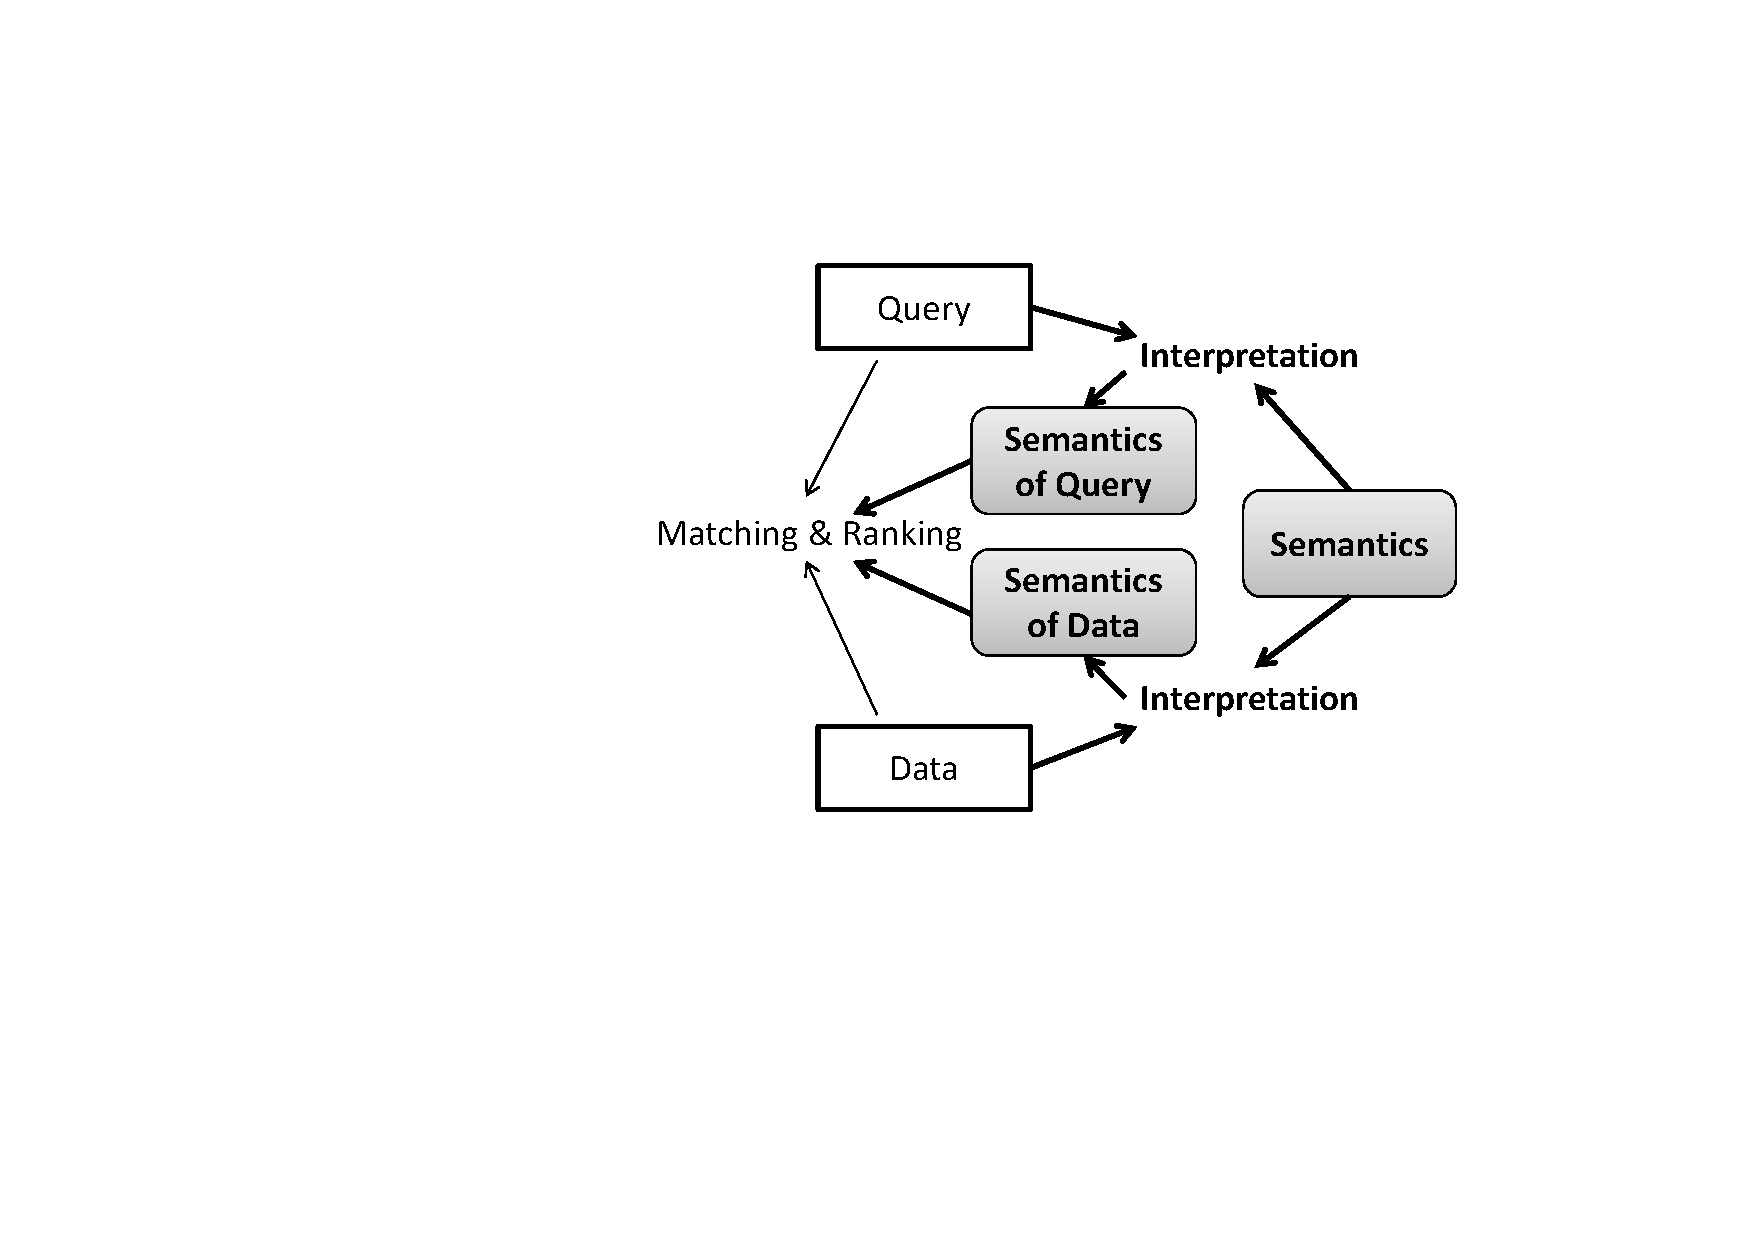
\includegraphics[width=0.35\textwidth]{figs/semsearch.pdf}
	\caption{Semantic Search.}
	\label{fig:semsearch}
\end{figure}

Basically, \emph{search} can be characterized by three components, namely the \emph{data}, the \emph{query} and the \emph{matching} framework for computing results from the data for a given query. This is illustrated in the left portion of Fig.~\ref{fig:semsearch}. One main characteristic of search concepts is its emphasize on end users. That is, search typically involves intuitive interfaces targeting users, who may do not possess knowledge about the domain, the data and structured query languages. The query inputs that can be obtained from these interfaces are often ambiguous. That is, they allow for many possible \emph{interpretation}s, which in turn, yield many possible results that vary in relevance w.r.t.~ the intended query intent. 
% Because end users are often only interested in the few best results, 
\emph{Ranking} is an essential component in search that aims to address this, i.e. to distinguish results in terms of relevance. Basically, matching can be conceived as the task of identifying matches whereas ranking is more specifically about the degree of matching.   

\emph{Semantic search} is a concept widely used by different communities to refer to search approaches that broadly speaking, use semantics to improve the search experience. Considering the core search tasks, semantics has been used to obtain a better understanding of the data and query as well as to improve matching and ranking based on that (see Fig.~\ref{fig:semsearch}). There are exist different notions of semantics. One the one hand, there are proposals for using the semantics of words captured as latent concepts (e.g. inferred through Latent Semantic Indexing~\cite{DBLP:conf/sigir/Hofmann99}) or latent topics (e.g. inferred through Latent Dirichlet Allocation~\cite{DBLP:conf/sigir/WeiC06}). While these models only implicitly capture the semantics in terms of some latent, unknown dimensions, there are also explicit models of semantics. For instance, Explicit Semantic Analysis uses Wikipedia articles, categories, and relations between articles to capture semantics in terms concepts, which are then used for concept-based IR~\cite{DBLP:journals/tois/EgoziMG11}. Other explicit models of semantics (henceforth called \emph{semantic models}) include thesauri, the terminological part (TBox) of ontologies and data schemas. While these models capture semantics at the conceptual level, there are also \emph{semantic data} capturing the semantics of individual entities. To accommodate the wide range of semantic search approaches that exist, we formulate the following general notion of semantic search:

\begin{definition} \emph{Semantic search} is a search paradigm that makes use of explicit semantics to solve core search tasks, i.e. to use semantics for interpreting query and data, matching query against data and ranking results. 
\end{definition}

While all semantic search approaches involve some kinds of explicit semantics, the retrieval contexts and the specific semantic models used to deal with the meaning behind the query intent and data vary. In particular, we identified the following aspects, based on which we will characterize and distinguish existing solutions:

\begin{itemize}
\item the type of targeted \emph{information needs},  
\item the representation of information resources (\emph{data}), 
\item the representation of the information need (\textit{query}) or respectively, the underlying method for querying the data (querying paradigms), 
\item the \emph{semantic models} used to understand and to represent the meaning behind query and data, 
\item the framework for \emph{matching} queries against data, which also involves \emph{interpreting} the data and query intent as well as \emph{ranking} the results.  
\end{itemize}

For instance, we can look at the differences in the data to arrive at the distinction between document retrieval and data retrieval, two major research directions in search that mark the borders of large communities. 

\textbf{Document Retrieval:} The IR community targets the document retrieval context where results are retrieved from a collection of documents (primarily textual data). Semantic search of this type is different from standard document retrieval approaches in the use of semantics. The traditional type of semantic models used here are thesauri that are employed to interpret the terms in the textual representation of queries and data. Recently, semantic data such as RDF resource descriptions have also been employed to interpret query and documents in terms of real-world entities and their relations. 

\textbf{Data Retrieval:} Querying entities and their relations is a core problem in database research. As opposed to the hidden semantics of textual content in documents, information about entities and their relations are explicitly available in this setting -- either directly as semantic data in RDF or as some kinds of structured data that can be converted to RDF. Thus, understanding the semantics of the underlying data is not the problem here. However, as opposed to standard data retrieval that is based on structured query languages, intuitive query interfaces are needed in the search context. This leads to the issue of ambiguity. Hence, semantic search approaches of this type have to deal with the resulting problems of interpreting the query intent and ranking the many possible results. 
%Just like in the document context, the goal here is to enable easy access to the most relevant results. Especially in the Semantic Web community, solutions targeting this problem are also referred to as semantic search because they use semantic data to interpret the query intent and to rank results. 

%In this section, we establish the main dimensions in which existing solutions vary and then discussed them in more detail in the subsequent sections. 
% and then, provide a taxonomy of semantic search approaches. We focus on approaches studied by researchers in the Semantic Web community that explicitly target semantic search. Selectively, we also point out works from the IR and database communities that deal with the same problem. 
%Search is about retrieving information that are relevant with respect to a given information need. 
%Generally speaking, approaches that fall under the category of \emph{semantic search} use semantic data for representing information and (or) semantic models for interpreting the data and information needs. 

More fine-grained than this general breakdown into document and data retrieval, Fig.~\ref{fig:semsearch_detailed} illustrates the specific differences in queries, data, semantics, results (corresponding to information needs) and solutions for the subproblems that distinguish existing semantic search approaches. We can see that central to semantic search is the use of semantics (depicted as gray boxes in Fig.~\ref{fig:semsearch_detailed}). In particular, semantic resources represented by lexical models, knowledge models as well as semantic data and metadata are used for the subproblems of understanding raw data (e.g. text) and queries. The resulting semantics of data and queries are then employed for solving the subproblems of matching and ranking.   
  
%We will now discuss them along these aspects. 

\begin{figure*}[tbh]
	\centering
		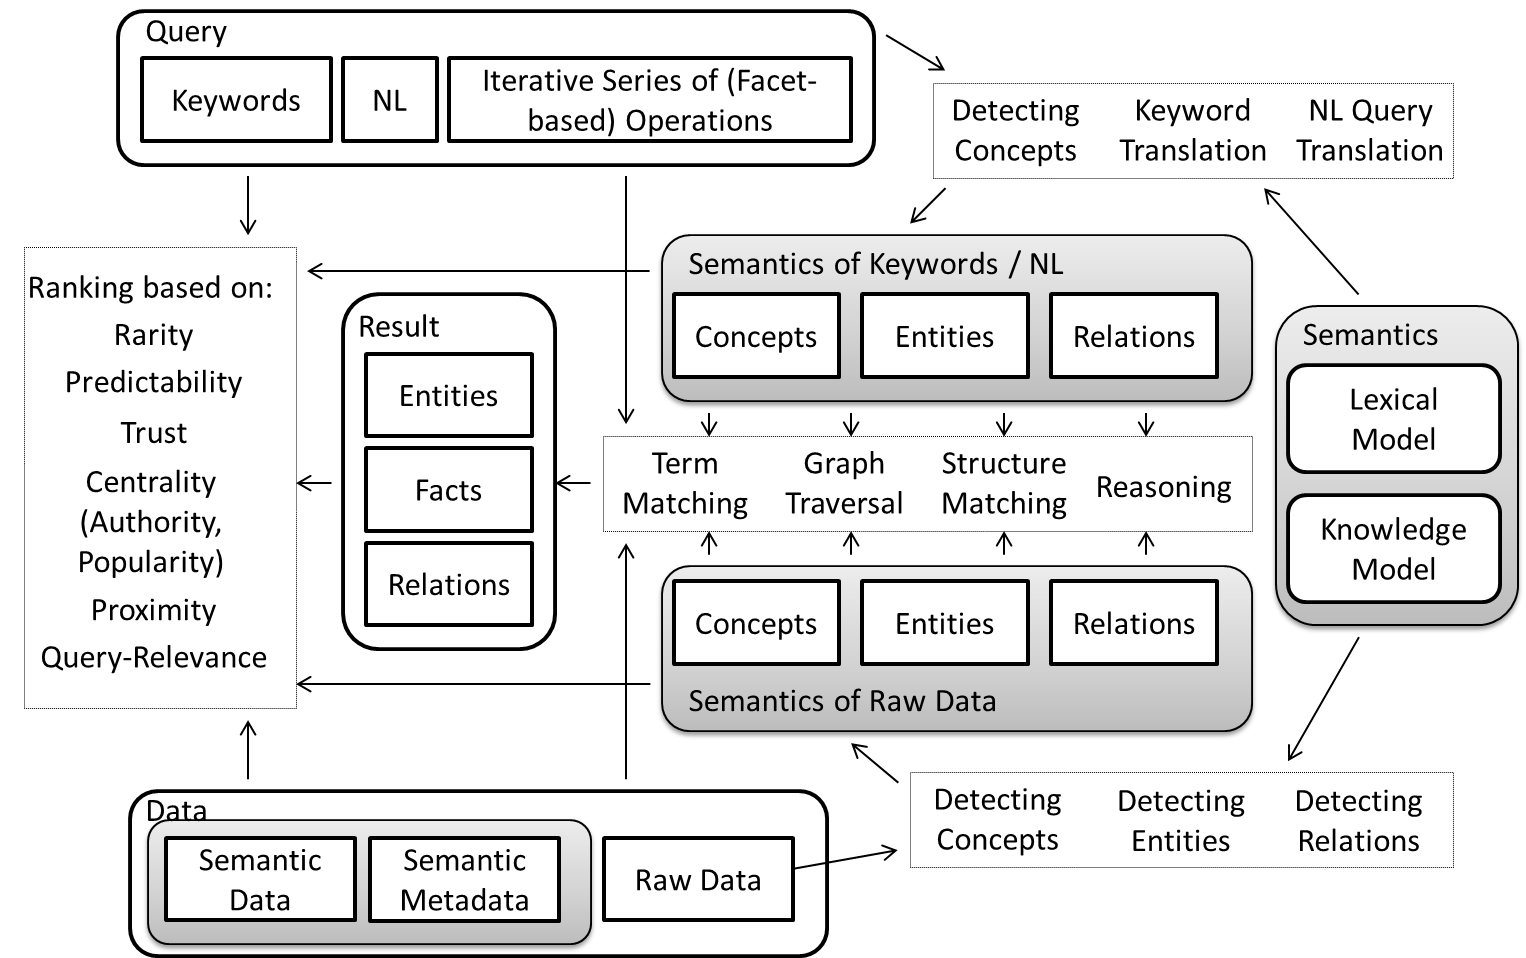
\includegraphics[width=0.75\textwidth]{figs/semsearch_detailed}
	\caption{Overview of Semantic Search Approaches.}
	\label{fig:semsearch_detailed}
\end{figure*}

\section{Information Needs}\label{sec:needs}

The main motivation for semantic search is to go beyond the relatively frequent but simple queries currently supported by existing Web search solutions to solve the long-tail queries representing rather complex information needs. But also for simple queries, semantic data have proven to be valuable. Instead of showing documents, semantic data are used by commercial Web search engines to create rich snippets for Web pages, or to deliver direct answers, e.g a specific address for a query mentioning ``location'' and a named entity such as ``Yahoo! Research Lab Barcelona''. We will now discuss several common types of queries and the information needs behind them, from the more simple entity queries to complex relational and analytical queries. 

\subsection{Entity Search} Most queries on the Web ask for pages representing entities such as companies or people. They are used to obtain entry points, while additional navigation and browsing are still required to satisfy the actual information need. Thus, in the IR context, these queries are also referred to as navigational queries. Recently, semantic data embedded in Web pages have been exploited to address this type of queries. This was pioneered by Yahoo! in their SearchMonkey program, and later adopted by Google to present rich entity snippets\footnote{Google Rich Snippets} as answers to this kind of queries. As an example, Fig.~\ref{fig:semantic_layer} illustrates the entity search functionalities provided by Yahoo!. Not only there are Web pages but also entity descriptions appear as results. These descriptions are directly retrieved from semantic data (in this case, a dataset about music artists and their albums). Instead of searching over a collection of documents, semantic search engines such as Falcons~\cite{DBLP:journals/ijswis/ChengQ09} and Sig.ma~\cite{DBLP:journals/ws/TummarelloCCDDD10} use semantic data only, and return entity descriptions in RDF as results. Examples for this type of queries include the one asking for ``young scholars in Germany'' already mentioned before, or the query ``Researcher Thanh Tran'' depicted in the top left portion of Fig.~\ref{fig:matching}. Results for queries of this type comprise one or several entities. 
	 
\subsection{Factual Search} While results to the previous type of queries presented to the users are either some entity descriptions or Web pages about entities, the information needs behind this type of search requests require specific information from these descriptions and pages, respectively. Many searches on the Web for instance, aim at finding the ratings of restaurants, or the phone number of a particular person. To continue with our example, users may directly ask for ``the birth place of young scholars in Germany''. Direct answers to this type of queries are supported by WolframAlpha\footnote{\url{http://www.wolframalpha.com/}} and True Knowledge\footnote{\url{http://www.trueknowledge.com/}}, or the various research prototypes such as Hermes~\cite{DBLP:journals/ws/TranWH09} or AquaLog~\cite{DBLP:journals/ws/LopezUMP07}. Since factual search is mostly about facts that correspond to attribute values of entities, it is often regarded as a particular type of entity search. In this survey, we do not further distinguish this from the general entity search task. 
 
\subsection{Relational Search} The information need here goes beyond single entities and their factual information. Answers to queries of this type comprise several entities and relationships between them. Hence, processing these queries requires some understanding of relations between entities. For instance, the example presented in the introduction about 32 year old computer scientists requires knowledge about their \verb+lives in+ and \verb+birth place+ relations to some locations. Relations may be explicitly specified as part of the keyword or NL query, and entities satisfying these relation constraints can be computed using SemSearchPro~\cite{DBLP:journals/ws/TranHL11} or AquaLog~\cite{DBLP:journals/ws/LopezUMP07}. 

Other systems such as NAGA~\cite{DBLP:conf/icde/KasneciSIRW08} also support searches where relations to be considered are not explicitly mentioned in the query, or simply \emph{unknown}. They address information needs that involve finding how some entities are related to some other entities. The interesting part of the results here are thus not the entities, but the relationships between them -- also referred in literatures as semantic associations (direct connection) or property sequences (indirect connections, i.e. path)~\cite{DBLP:conf/www/AnyanwuS03}. An example for this type of query asking for paths between ``Peter Mika'' and ``Thanh Tran'' is depicted in the top right portion of Fig.~\ref{fig:matching}.

Even though Yahoo! entity search as shown in Fig.~\ref{fig:screenshot_yahoo} does not directly search for relations, it can be seen on the left portion that relations between entities captured in semantic data constitute valuable information for suggesting related entities. Searching for known relations or unknown relations is supported by the Information Workbench\footnote{\url{http://iwb.fluidops.com}}, a commercial adoption of SemSearchPro. On the bottom part of Fig.~\cite{fig:screenshot_iwb}, we can see results returned to a query that specifically asks for entities connected through the \verb+producer+ relation. When relations are not explicitly given in the query but only entities and (or) concepts, this system is also able to explore paths between them. However, this system does not directly return relationships and paths in the data as results, but structured queries representing interpretations of the entered keywords -- a querying paradigm we will discuss in the next section. 


 
	
\subsection{Analytical Search}
Beyond the common searches for entities and relations, which form the focus of this survey, there are also information needs, which can only be addressed when some additional analyses are performed on top of the data. Generally speaking, any kind of additional computation may be applied to the data and results for the purpose of analytical search. Analytics often found in semantic search engines are supported through simple sorting and averaging, more sophisticated statistical and mathematical models, or some form of Machine Learning based inductive reasoning or logic-based deductive reasoning. For instance, WolframAlpha is advertised as a computation engine because it applies different kinds of mathematical models to compute answers to queries, whereas True Knowledge uses an inference engine to perform temporal and geospatial reasoning. 



\begin{figure}
	\centering
		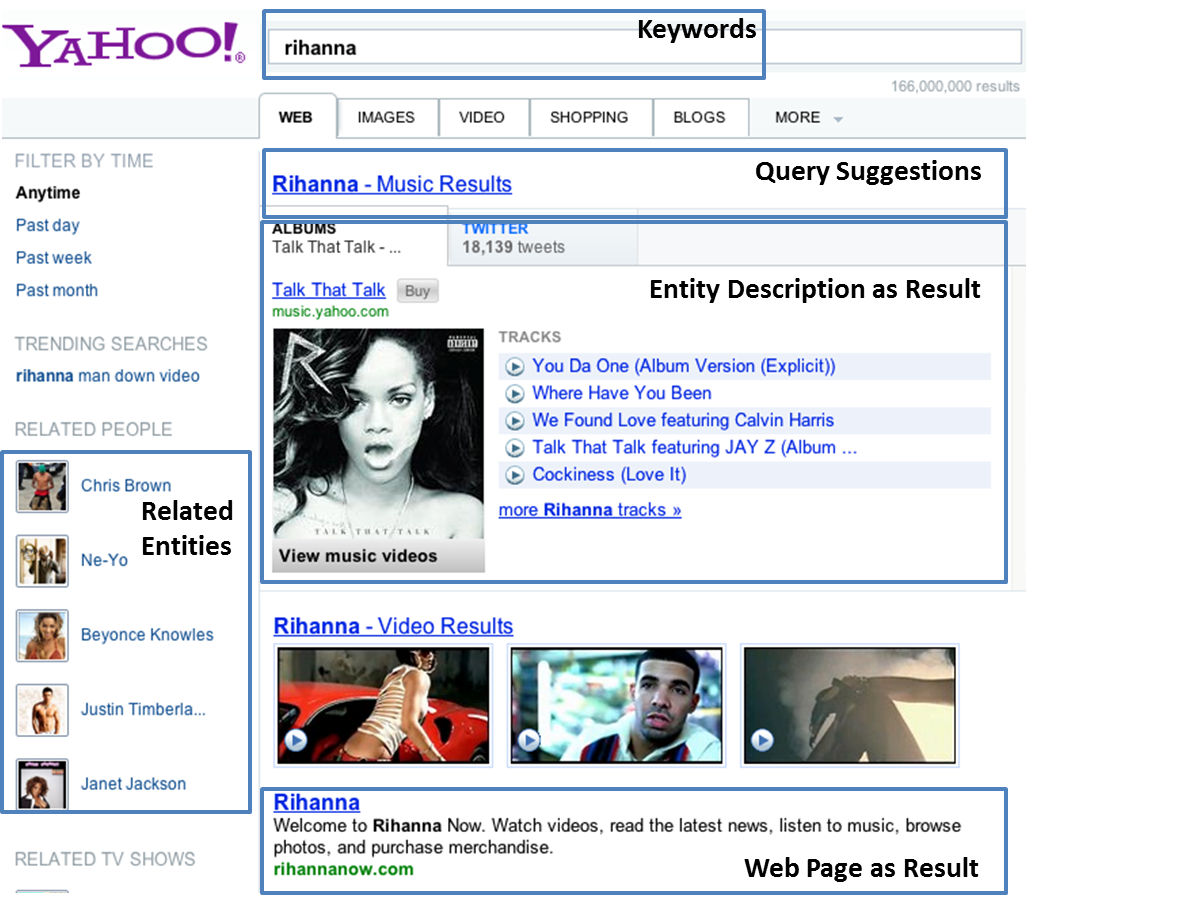
\includegraphics[width=0.5\textwidth]{figs/screenshot_yahoo}
	\caption{Entity search with Yahoo!.}
	\label{fig:screenshot_yahoo}
\end{figure}


\section{Querying Paradigms}\label{sec:querying}
Typically, addressing complex needs requires the expertise of technical users who know the underlying data and schema and use them to formulate questions as structured queries. However, search is commonly seen as an end-user oriented paradigm, which instead of using structured query languages, involves intuitive and easy-to use access interfaces. The three main interfaces studied for semantic search are based on keywords, NL, and facets. Often, a combination of these paradigms, e.g. keywords and facets, is used to support an iterative search process where instead of constructing the query at once, the user modifies the query and results respectively, through a series of operations.    


\subsection{Keyword Search} Expressing the information needs as keywords is a paradigm that is not only popular for Web search but also widely adopted by the new breed of semantic search solutions. Most engines focusing on entity search such as Falcons~\cite{DBLP:journals/ijswis/ChengQ09} and Sig.ma~\cite{DBLP:journals/ws/TummarelloCCDDD10} feature a keyword search interface. Keywords can also be used to formulate more complex relational searches. Addressing this scenario, engines such as Hermes~\cite{DBLP:journals/ws/TranWH09}, SemSearchPro~\cite{DBLP:journals/ws/TranHL11}, TASTIER~\cite{DBLP:conf/sigmod/LiJLF0} and IBM's AVATAR~\cite{DBLP:conf/sigmod/KandoganKRVZ06} retrieve entities matching keywords, and search for relations between them in the data. 
	
	
\subsection{NL Search} This is the other paradigm for users to express their needs using their own words. Traditionally, it has been used to pose complex questions against expert systems built for specific domains. Recently, NL interfaces have proven to be also applicable and useful for the multiple domains setting and especially for Web search -- as demonstrated by commercial engines such as WolframAlpha, True Knowledge and Apple's Siri\footnote{\url{http://en.wikipedia.org/wiki/Siri_(software)}}. 	
	

\subsection{Faceted Search} Instead of formulating the entire query at once, \emph{faceted search} supports an iterative process of querying, browsing and query refinement. This belongs to the broader category of approaches called \emph{exploratory search}, which assumes that users do not precisely know how or what to search and thus, combines querying and browsing strategies to enable learning and investigation. Upon the initial search performed by the user (e.g. using keyword search), faceted search systems~\cite{DBLP:conf/dexa/WagnerLT11,DBLP:conf/semweb/FerreH11,DBLP:conf/esws/HeimEZ10} present results as well as facets representing attributes and relations that are applicable for refining (or simply, are related to) the current results. These facets can then be used to browse, to refine or to expand the results (i.e. to modify the query, respectively). Microsoft's EntityCube\footnote{\url{http://entitycube.research.microsoft.com/}} for instance, returns entities upon users' keyword search requests along with relations and attributes of these entity results as facets. Parallax\footnote{\url{http://www.freebase.com/labs/parallax/}} is another commercial faceted search solution (from Freebase, now Google) that enables a combination of search, intelligent result visualization and facet-based browsing. 

While most faceted search solutions focus on browsing and refining results of entity queries, faceted search in principle can also be used to address complex needs. For instance, gFacet~\cite{DBLP:conf/esws/HeimEZ10} supports relational search through the construction of complex facet graphs representing different types of entities and relations between them. Fig.~\ref{fig:screenshot_iwb} shows the faceted search feature from the Information Workbench. Every column in the result table captures one particular type of entities and this system shows facets for every type that appears in the results (e.g. Fig.~\ref{fig:screenshot_iwb} shows facets for column 1). Hence, entries in every column (representing a partial result and a query part, respectively) can be refined or expanded. For instance, the column of singles shown in Fig.~\ref{fig:screenshot_iwb} can be further refined to contain only those connected with \verb+Freddie Mercury+ through the \verb+writer+ relation. 

\subsection{Iterative / Exploratory Search} 
While faceted search is the most popular paradigm in the industry, there are other exploratory search interfaces that support an \emph{iterative search} process. Instead of showing facets as users type, also \emph{completions} of the single user keywords (term completions) or of the entire query representing the full query intent (query completions) have been proposed. One example system supporting this is the Information Workbench shown in Fig.~\ref{fig:screenshot_iwb}, which presents terms matching the current tokens entered by the users, as well as full interpretations of the entire query. For ``queen single'', the interpretations shown indicate that the query intent may be something matching the word ``queen'' that is of the type \verb+single+, or something that is of the type \verb+single+, which is produced (or written) by something else matching the word ``queen''. Google, Freebase\footnote{\url{http://www.freebase.com/docs/suggest}} and True Knowledge also present possible interpretations of the query as the user type or after issuing a query. 

Instead query-based completions, also results matching the (possible interpretations of the) keywords provided so far have been presented (called result completions~\cite{DBLP:conf/esws/TranMH10}). For instance, ESTER~\cite{DBLP:conf/sigir/BastCSW07} shows entity search results matching the keywords as well as their facets (see CompleteSearch~\footnote{\url{http://www.dblp.org/search/index.php}}, which is an adoption of ESTER) whereas TASTIER~\cite{DBLP:conf/sigmod/LiJLF09} provides type-ahead search by finding complex (joins of) database tuples as the user types query keywords. With these systems, users can iteratively construct the query by selecting the presented completions and facets. VisiNav~\cite{DBLP:journals/ws/Harth10} goes beyond this selection-based interaction, allowing iterative query construction also via drag and drop. 	
	
\begin{figure}
	\centering
		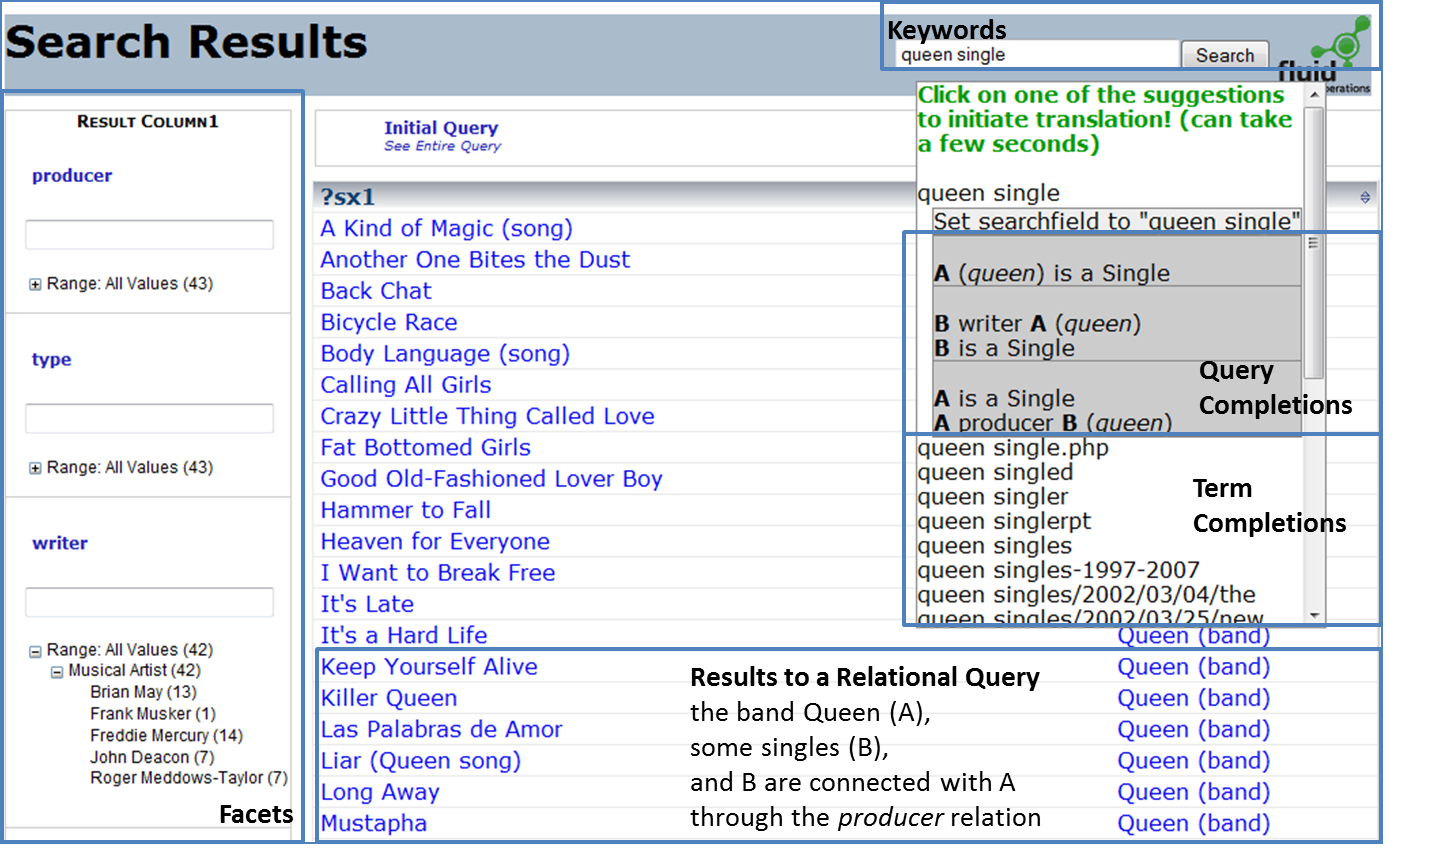
\includegraphics[width=0.5\textwidth]{figs/screenshot_iwb}
	\caption{Querying with the Information Workbench.}
	\label{fig:screenshot_iwb}
\end{figure}




\section{Data}\label{sec:data}
The information resources made available for search as well as any kind of additional background information used to improve the search experience, are kept and managed by the system as data. In semantic search solutions, data can be broadly categorized into two types, namely \emph{semantic data} and \emph{raw data}. 

Basically, semantic data describe real-world objects in terms of entities and their relations. Primarily, semantic data have been used to refer to RDF datasets, or instance data contained in ontologies represented in Semantic Web languages such as OWL (the Web Ontology Language, a logic-based W3C standard\footnote{http://www.w3.org/TR/owl-features/} for representing the semantics of vocabulary / schema elements) and RIF (the Rule Interchange Format, a W3C standard for representing and exchanging rules). However, different kinds of structured data actually correspond to this rather general notion of semantic data. In fact, large amounts of structured data formerly kept in hidden 
%XML or relational 
Web databases 
have been converted to and published on the Web as RDF data. Several semantic search systems have been built that specifically target the retrieval of semantic data. Instead of searching directly over semantic data, classic retrieval systems search over a raw data representation of information objects such as audios, videos, images and texts. For instance, document retrieval systems search for textual documents that are represented as bags of words. As opposed to semantic data, raw data do not explicitly capture the semantics of information resources in terms of entities and their relations. Thus, for supporting document (or image, video or audio) retrieval as semantic search, one core subtask is the recognition of named entity in the raw text. Named entity recognition and other data interpretation tasks such as relation extraction are performed to obtain a semantic data representation of raw data (also called \emph{semantic metadata}). 


\subsection{Semantic Data}  The most common type of semantic data used in semantic search systems is RDF. Basically, RDF is a graph-structured model, representing entities, their attributes, and relations between them as a set of triples. A visual illustration of such a \emph{semantic data graph} capturing information about two \verb+researcher+s, whose \verb+names+ are \verb+Thanh Tran+ and \verb+Peter Mika+, is depicted in the bottom portion of Fig.~\ref{fig:matching} 

This general graph-structured model can be used to capture structured data of different types. In fact, most of the data made publicly available on the Web and incorporated into semantic search engines such as Falcons~\cite{DBLP:journals/ijswis/ChengQ09}, Sig.ma~\cite{DBLP:journals/ws/TummarelloCCDDD10} and Hermes~\cite{DBLP:journals/ws/TranWH09} originate from relational or XML databases. XML elements can be represented as nodes, and their structure information can be captured as edges. Likewise, information contained in tuples of a relation database can be mapped to nodes, while foreign key relationships can be modeled as edges. In fact, the conversion of XML and relational data to a RDF semantic data graph can be accomplished by using mapping rules, and there exist many standards and tools for accomplishing that (e.g. see W3C RDB2RDF\footnote{\url{http://www.w3.org/2001/sw/rdb2rdf/}}). Represented as RDF, these and possibly other types of structured data also capture information about real-world objects in terms of entities and their relations. Hence, especially after their conversion to RDF, structured data are often synonymously referred to as semantic data. To capture this general notion of semantic data used in semantic search systems, we introduce the following definition: 

\begin{definition}
\emph{Semantic data} can be conceived as a graph, where nodes represent \emph{entities} and their \emph{attribute values}, and edges stand for \emph{attributes} of entities or \emph{relations} between entities. 
\end{definition}

In particular, this notion accommodates three main types of semantic data currently used in semantic search systems, namely (1) text-rich entity descriptions contained in structured document collections, (2) structured entity descriptions in RDF and (3) formal logic-based entity descriptions specified using expressive knowledge representation languages such as OWL. 

\textbf{Text-Rich Entity Descriptions:} This category of semantic data contains entities that are largely described through text, i.e. entity attribute values are composed of lengthy textual descriptions. Wikipedia is the most popular example that lies at this end of the spectrum of semantic data. While it is actually a collection of documents (i.e. contains mainly textual data), it fits the presented notion of semantic data because every Wikipedia page corresponds to an entity, and there are links between Wikipedia pages that can be seen as relations. In fact, exploiting this and other specific features of Wikipedia articles such as Infoboxes, a RDF dataset called DBpedia~\cite{DBLP:journals/ws/BizerLKABCH09} has been automatically derived from this collection. Wikipedia as a source of semantics is particularly popular for search systems that focus on expert search or entity search in general. It is used either to directly answer entity search queries or as background knowledge~\cite{DBLP:conf/cikm/KapteinSVK10,DBLP:conf/cikm/BronBR10}. 


\textbf{Structured Entity Descriptions:} This type of semantic data is ubiquitous on the Web, capturing information about real-world objects as RDF resource descriptions (or structured entity descriptions that can be directly converted to RDF). Through industry efforts such as Yahoo's SearchMonkey, Google's Rich Snippets and Facebook Like\footnote{\url{http://developers.facebook.com/docs/reference/plugins/like/}}, a large amount of RDF descriptions of resources such as restaurants and movies have been embedded into existing Web pages as RDFa. Besides, hundreds of large-scale RDF datasets have been made available on the Web. Started with the Linking Open Data, more and more data are made freely available on the Web and linked with other public datasets. Not only Web content providers but many companies, public institutions and national governments (US, UK etc.) are now actively publishing and linking RDF data on the Web (called Linked Data). Availably datasets can be subdivided into broad/domain-independent ones such as as DBpedia and Freebase\footnote{\url{http://www.freebase.com/}} or deep/domain-specific ones. Large domains covered by Linked Data today include government, health care, entertainment and geography.  


\textbf{Formal Entity Descriptions:} On the other end of the spectrum, there are more formal views on what constitutes semantic data. In particular, many researchers may argue that the reason why RDF, and other data models that are built upon a formal model of semantics, are actually called semantic data (instead of structured data) is because they can be exploited by a reasoning engine to infer new knowledge (i.e. the knowledge that is entailed by the semantics). While the formal model of semantics specified for RDF is relatively simple (consists only of a few inference rules), semantic data in some existing search systems are represented using more expressive knowledge representation languages such as OWL and F-logic~\cite{DBLP:conf/sigmod/KiferL89} (basically, a combination of logic and object-oriented frame-based languages). For instance, Serene~\cite{DBLP:journals/ws/FazzingaGGL11} makes use of facts that are captured as Abox assertions (i.e. instance data, as opposed to Tbox, the schema part) of an OWL ontology. ORAKEL~\cite{DBLP:journals/dke/CimianoHHMS08} searches over an F-logic knowledge base. However, while the use of formal semantics and reasoning has been investigated for some scenarios, it plays only a limited role in existing systems. The 
majority of approaches does not rely on reasoning. It seems that the research focus still lies in correctly understanding the ambiguous queries and data (namely, to interpret queries and data as elements of the semantic data model as defined above), while reasoning over semantic data may be beneficial but not essential yet. 

To sum up, a general notion of semantic data is employed in this work to consider all those systems, which capture the semantics of information resources and real-world objects as entities and relations. Often, these entities and relations are specified on the account of a formal data model with well-defined semantics (e.g. RDF, OWL, F-Logic). However, such a formal model is not strictly required (e.g. in the case of text-rich entity descriptions) and in particular, may not be exploited for reasoning. 
	
\begin{figure}[thb]
	\centering
		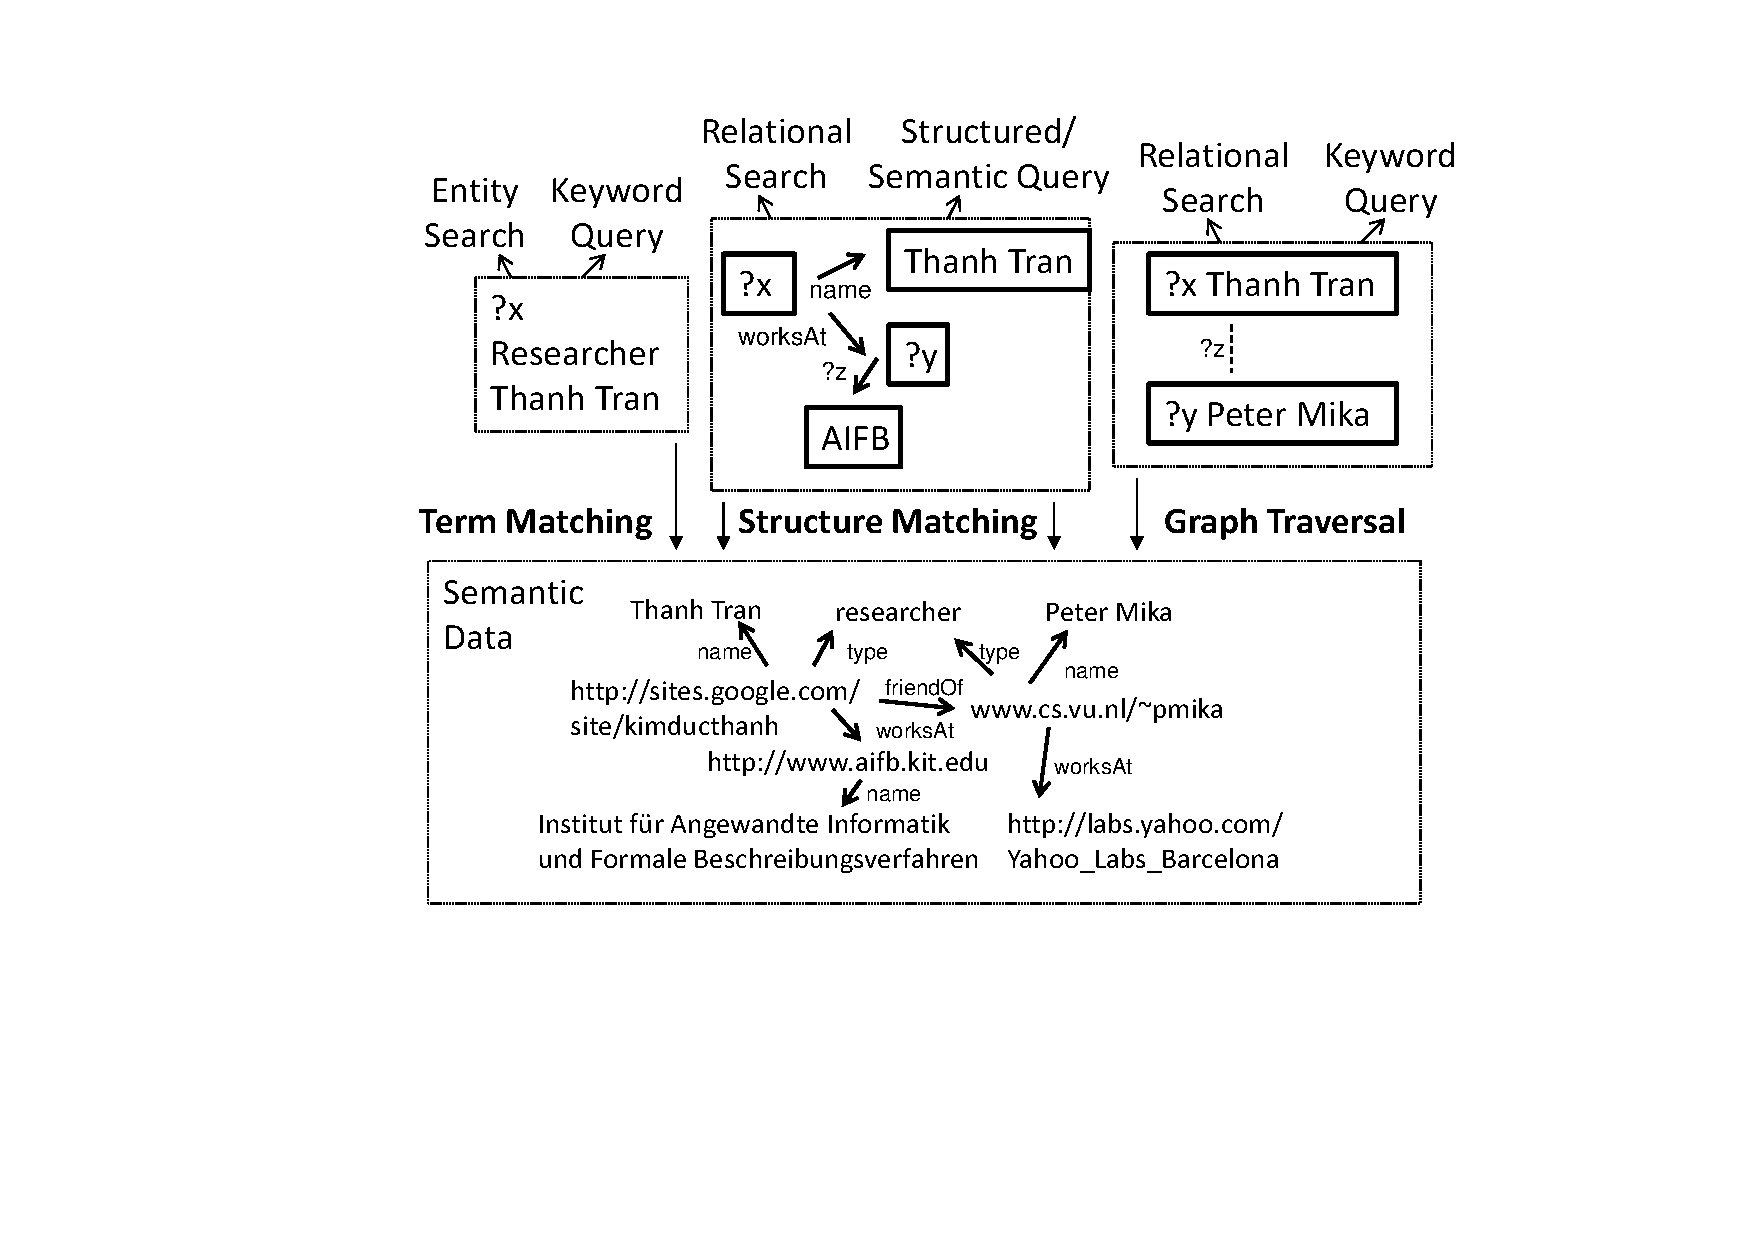
\includegraphics[width=0.5\textwidth]{figs/matching.pdf}
	\caption{Examples for semantic data, queries and matching techniques.}
	\label{fig:matching}
\end{figure}

There are engines operating directly on semantic data to provide direct answers (data retrieval systems). These are mainly systems, which provide search interfaces over RDF data and ontologies crawled from the Semantic web~\cite{DBLP:journals/ijswis/ChengQ09,DBLP:journals/ws/TranWH09,DBLP:journals/ws/HoganHUKPD11}, or structured databases that have been converted to semantic data graphs~\cite{DBLP:conf/sigmod/LiJLF09,DBLP:conf/sigmod/LiOFWZ08}. Besides them, there are also semantic search systems supporting the retrieval of documents or information objects in general. They employ semantic metadata, often in combination with the raw data representation of these objects. 
	
\subsection{Semantic Metadata}
Basically, semantic metadata is semantic data that captures information about the objects to be retrieved. Because it is clear from the context, these two terms are often used synonymously (in this work). Metadata include basic information about the objects such as \verb+author+ and the \verb+year+ it was published. Moreover, it may capture the semantics of the information contained in these objects. For instance, if a particular Web page is about a restaurant, its metadata may contain a structured description of that restaurant (as RDFa) corresponding to the text contained in the page. In fact, one main challenge in semantic search is to interpret the semantics behind the content of information objects and to represent it as semantic metadata. Not only entities may be recognized but for instance, the content of a document may be interpreted as referring to a \verb+meeting+ with the two \verb+researchers+ \verb+Peter Mika+ and \verb+Thanh Tran+ as \verb+participants+. Semantic metadata representing the content may also be manually produced and embedded into the objects. Recently, several industry projects such as Google Rich Snippets and Yahoo! SearchMonkey actively target this development, providing incentives for site owners to embed RDFa or other kind of semantic metadata into their Web pages. Complementary to this,  schema.org\footnote{\url{http://schema.org/}} is an initiative promoted by major Web search companies (Google, Microsoft, Yahoo!) aiming at the provision of a common vocabulary that can be used by site owners to capture their data. In this regard, we note that while Wikipedia can be conceived as semantic data (with pages corresponding to entities), a more typical viewpoint is to consider it as a collection of documents that are manually associated with metadata: every page is associated with a set of categories and exactly one entity (the entity it is about).  




While the amount of available metadata is increasing, it is still too sparse to cover all information needs. Thus, metadata is mostly used as additional information that can help to improve standard search over raw data~\cite{DBLP:journals/tkde/CastellsFV07,DBLP:journals/ws/FernandezCLVCM11}. Search over raw data can also be seen as a fall-back solution for cases where metadata cannot completely satisfy the information need. There exist also 	proposals for ontology-based IR, which completely rely on metadata~\cite{tran2007expressive}. In this case, the retrieval of documents is formulated as a data retrieval task, where data about the documents (metadata) are returned as direct answers. 

\section{Semantics: Semantic Data and Semantic Models}\label{sec:semantics}
\begin{figure}[thb]
	\centering
		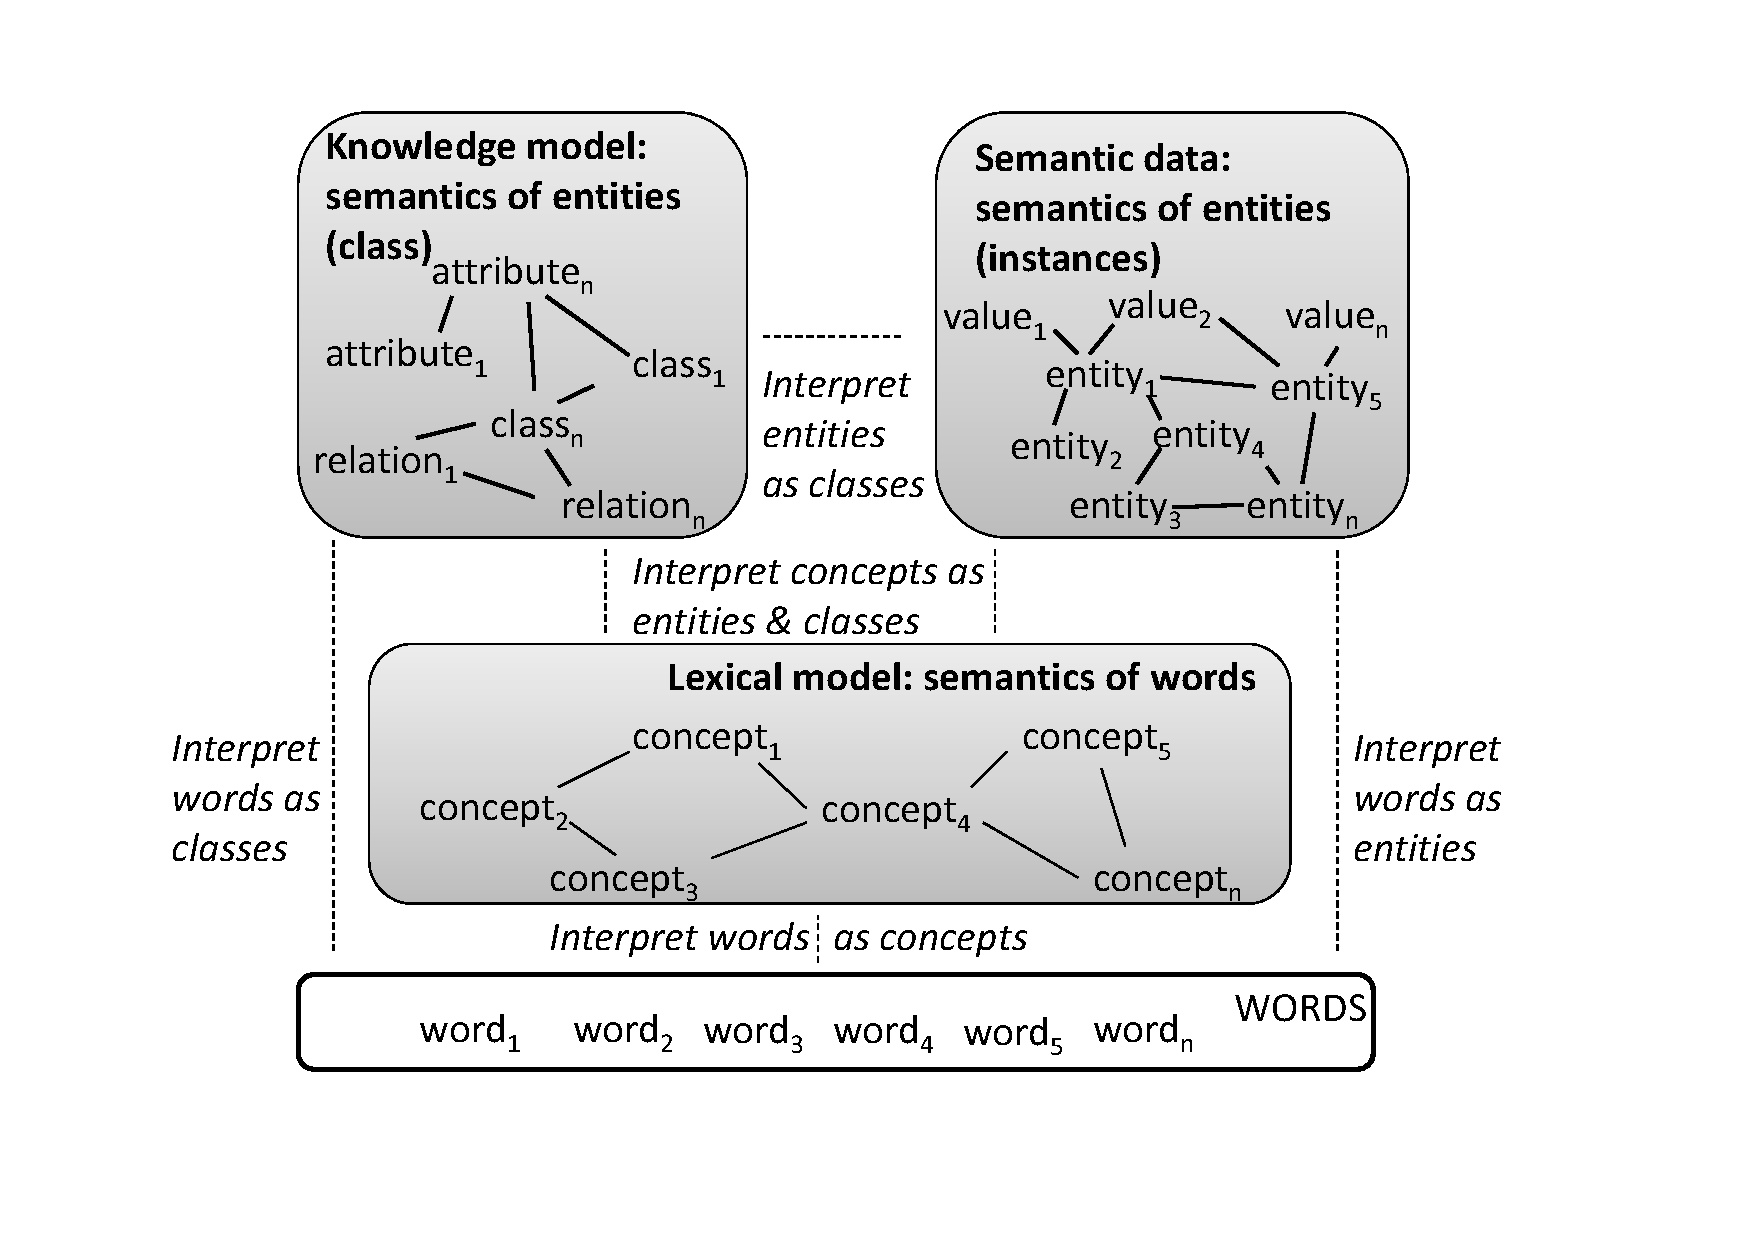
\includegraphics[width=0.5\textwidth]{figs/semantic_layer.pdf}
	\caption{Words, concepts and entities.}
	\label{fig:semantic_layer}
\end{figure}

As discussed, central to semantic search system is the use of semantics. The color highlighting (gray) in Fig.~\ref{fig:semsearch_detailed} indicates that a main source of semantics is the \emph{semantic data} itself. That is, semantic data can be used directly to answer queries (i.e. by matching queries against semantic data), or as a semantic resource to interpret raw data and queries (as we shall see in more detail in subsequent sections). More specifically, Fig.~\ref{fig:semantic_layer} shows that in the textual raw data context, these semantics can be used to interpret words in terms of entities and relations. It also shows the other sources of semantics called semantic models. Broadly, \emph{lexical models}, which capture semantics at the level of words in terms of concepts, can be distinguished from \emph{knowledge models}, which capture real-world knowledge in terms of entity classes, relations, and attributes. 

We have discussed semantic data as one source of semantics in the previous section. In this section, we provide an overview of the semantic models used by current systems, and subsequently, present a notion of semantics that combines the instance-level semantics captured by the data and the schema-level (conceptual) semantics captured by the semantic models. 

\subsection{Knowledge Models} While semantic data capture concrete entities (instances), these are abstract models of knowledge, basically representing classes of entities, attributes associated with these classes, and relations between classes. This is visualized in the top left portion of Fig.~\ref{fig:semantic_layer}.  

Different models, which vary in the degree of formality and expressiveness have been used by different communities for semantic search. For instance, the model used by ORAKEL for NL question answering is captured by the Tbox portion of an ontology and consists of classes (also called concepts) that are ordered in a subsumption hierarchy and are connected through relations. Range and domain information are captured as restrictions on the relations. As shown for Serene~\cite{DBLP:journals/ws/FazzingaGGL11}, expressions more complex than these restrictions can be added to capture the semantics of concepts to reflect either general knowledge (such as the knowledge encoded in Wikipedia)
or specific knowledge of a domain. Because the ontology models used in these systems are represented using the logic-based formalisms F-logic or OWL (description logic, DL), they can be seen as \emph{logical theories} with well-defined formal semantics. 

Also, \emph{conceptual graphs} (CGs) have been employed for representing ontology models, and used for the tasks of NL questions interpretation and answering~\cite{DBLP:conf/aswc/CaoCT08} as well as for interpreting and representing documents~\cite{DBLP:conf/iccs/ComparotHH07}. CGs combine the intuitiveness of graph-based languages and the formal foundation of logics, enabling the modeling of knowledge in terms of concepts and their relations and its mapping to different formal languages. Corese~\cite{DBLP:conf/ecai/CorbyDF04} uses CGs as an internal model (to take advantage of previous work on CGs in the KR community), which however, are then translated to RDFS to conform with this more commonly used standard language for representing RDF schemas. 

Closer to the end of linguistic models discussed next are knowledge models that consist of concepts only. For instance, C-Search~\cite{DBLP:conf/esws/GiunchigliaKZ09} encodes knowledge as concepts expressed in propositional DL. This DL enables the representation of complex concepts as a conjunction or disjunction of atomic concepts. However, it does not support relations. 
% (also called roles) but the specification 

		
\subsection{Lexical Models} The use of concepts has already been investigated in the early years of IR research~\cite{DBLP:conf/sigir/Giger88}. Different to knowledge models, which capture semantics in terms of real-world entities and their relations, the models employed there are lexical in the sense that they capture semantics at the level of words. While concepts in knowledge models stand for classes of real-world entities, concepts in lexical models correspond to \emph{senses of words}. Lexical concepts are more general such that they may refer to entities, classes, relations, attributes, or other senses of words. While these different ``types'' of senses are not explicitly distinguished like in a knowledge model, concepts can be organized along lexical relationships in a lexical model. 

\emph{Thesaurus} 
%(often, \emph{lexicon} is also used as synonym) 
is a popular lexical model that has been extensively used for document retrieval in IR, which basically, groups words together according to their semantic similarity. Each group represents a different word sense. In practice, lexical databases also considered as thesauri such as WordNet, or thesauri used in classic IR systems~\cite{DBLP:conf/sigir/Giger88}, not only capture senses (concepts) and their lexical variants, but also relationships between them such as synonym, broader, narrower and related. This is illustrated in the bottom part of Fig.~\ref{fig:semantic_layer}. 


\subsection{Semantics} 
Based on the above discussion, we introduce a general notion of semantics that can be used to characterize the different types of semantic search systems.

\begin{definition} The \emph{semantics} of queries and data are captured by semantic search systems in different ways. Semantics can be represented (1) as word senses that are organized through lexical relations between words (\emph{lexical model}), (2) as specific knowledge about concrete entities, i.e. specific attribute values and relations between entities (\emph{semantic data}) or (3) as general knowledge about classes of entities, class attributes, and relations between classes (\emph{knowledge model}). 
\end{definition}

A prominent example that can be used to illustrate these many aspects of semantics is Wikipedia. As discussed, it has been used as semantic data to answer entity search queries, and converted to a semantic dataset called DBpedia~\cite{DBLP:journals/ws/BizerLKABCH09}. The Wikipedia categories of pages have been treated as classes and used to construct hierarchies of classes in an ontology called YAGO~\cite{DBLP:conf/www/SuchanekKW07}. Wikipedia is also used as a source for Explicit Semantic Analysis (ESA)~\cite{DBLP:journals/tois/EgoziMG11}, where every Wikipedia page is regarded as a concept. Because ESA does not distinguish entities from classes, the concepts here can be seen as capturing word senses. Thus, Wikipedia pages and links constitute a lexical model in this context. 

\subsection{Focus: Semantics of Entities \& Relations} 

The discussion of semantics so far focuses on entities and simple (binary) relations between them. Yet, the kind of semantics that can be expressed is only limited by the knowledge representation (KR) languages. There exist very powerful KR formalisms and many of them have been incorporated to perform document retrieval (already in the early years of IR~\cite{DBLP:conf/sigir/Rijsbergen89}) and to represent complex queries and knowledge used in NL question answering~\cite{DBLP:journals/tkde/VassiliadisTK94} (in the early years of expert systems). For instance, the employed formalisms have been used to represent temporal or fuzzy aspects of world knowledge. However, there are practical reasons why the focus of current research (and this paper) is set on simple descriptions of entities (via attribute and binary relations). On the one hand, 
%most queries on the Web ask about entities and their relations. That is, 
most common queries as well as a large part of queries in the long tail of Web query logs 
%can be addressed using semantics about 
are about entities and relations (i.e. they are of the types entity, factual or relational queries). More importantly, the bottleneck is actually the availability of data. It became evident that manually capturing the content of documents as complex logical formulas does not scale. Extracting entities and relations from documents at high quality still remain hard problems, representing the limits of what can be done automatically by data extraction technologies. Also, most of the data residing in databases nowadays are mainly about entities and their relations. 


%\dtr{maybe also discuss the difference to XML retrieval, which merely use structure information for ``focused'' retrieval: retrieve components of the structured XML documents that match the query: The focus on the semantics of entities and relations also marks the boundary between semantic search and XML document retrieval. }

 
%\section{Interpretation}
\begin{figure*}[htb]
	\centering
  \subfloat[Detecting concepts.]{\label{fig:detecting_concepts}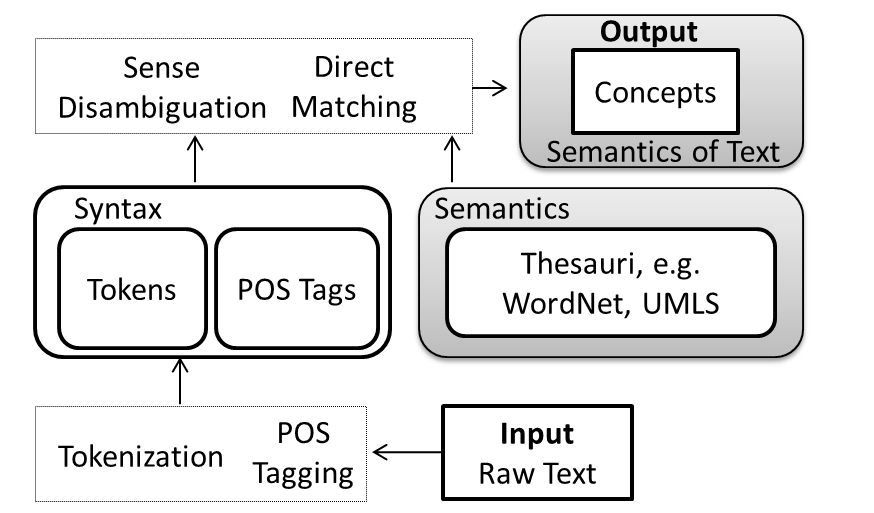
\includegraphics[width=0.34\textwidth]{figs/conceptextraction}}
  ~ %add desired spacing between images, e. g. ~, \quad, \qquad etc. (or a blank line to force the subfig onto a new line)
  \subfloat[Detecting entities and relations.]{\label{fig:detecting_data}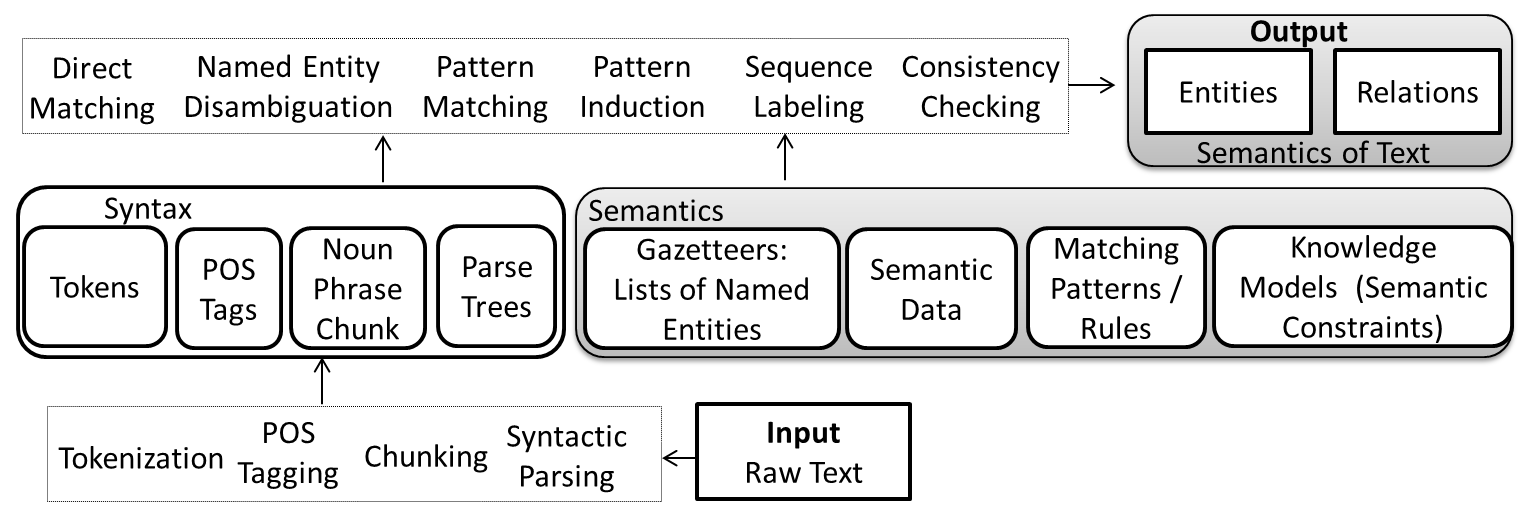
\includegraphics[width=0.6\textwidth]{figs/dataextraction}}
  \caption{Detecting concepts, entities and relations.}
  \label{fig:extraction}
\end{figure*}

\section{Content Interpretation}\label{sec:content}
	
One crucial task in supporting semantic search over documents is to obtain a richer understanding and representation of the document collection. Instead of a the typical bag-of-words model used in classic IR, the goal is to capture the content of the documents as entities, concepts and relations, i.e. as semantic data or elements of a semantic model. In fact, there is a dedicated area of research focusing on this problem of knowledge extraction from text. Problems that have been studied include named entity recognition, semantic role labeling and relation extraction. For an overview of solutions proposed in this area, we refer the interested readers to surveys specifically focused on this problem~\cite{DBLP:journals/tkde/ChangKGS06}. Here, we discuss the kind of knowledge extraction that has been performed for the purpose of semantic search. 

\subsection{Detecting Concepts in Text} This problem and the tasks carried out to solve it are illustrated in Fig.~\ref{fig:detecting_concepts}. Concepts are especially needed for supporting what is known as concept-based IR. 

Documents have been analyzed to extract concepts for the task of modeling documents as conceptual graphs~\cite{DBLP:conf/iccs/ComparotHH07}. For C-Search~\cite{DBLP:conf/esws/GiunchigliaKZ09}, which represent documents as DL concepts corresponding to WordNet senses, the authors identify words in documents matching Wordnet senses (i.e. direct matching), and uses part-of-speech (POS) tagging information and Wordnet, as lexical database of senses and word-level relationships, to perform word sense disambiguation. While words are mapped to atomic concepts, phrases are represented as complex concepts using DL formulas~\cite{DBLP:conf/esws/GiunchigliaKZ09}. Especially in the biomedical domain, the use of thesauri concepts for interpreting and representing documents is very common~\cite{DBLP:conf/trec/TrieschniggKS06,DBLP:conf/trec/ZhouYTS06}. For instance, the Unified Medical Language System and a gene-thesaurus have been used to identify multi-word terms and to map synonymous words to one concept~\cite{DBLP:conf/trec/TrieschniggKS06}. The concepts were identified simply by matching document words to thesaurus terms.
	
	
\subsection{Detecting Entities \& Relations in Text} For extracting entities and relations, the large body of research work on named entity recognition and relation extraction has been leveraged by existing semantic search solutions. One of the platforms, which is frequently used by semantic search systems for extracting semantic data and
automatically annotating document collections at a large scale is KIM~\cite{KIM DBLP:journals/ws/KiryakovPTMO04}. IBM's AVATAR~\cite{DBLP:conf/sigmod/KandoganKRVZ06} makes use of UIMA, a framework of annotators that can be configured in a pipeline to analyze and extract data from text. There is a another work from IBM, which focuses on extracting named entities and relations from text and using them for more precise search (employing XML fragments as queries~\cite{DBLP:conf/sigir/Chu-CarrollPCFD06,DBLP:conf/cikm/Chu-CarrollP07}).

An overview of tasks involved in detecting entities and relations are shown in Fig.~\ref{fig:detecting_data}. As for most text interpretation tasks, a syntactic analysis of the text is needed. In this case, the typical analysis includes tokenization, POS tagging, chunking sentences into noun phrases, and some data extraction systems even derive entire parse trees from the text. Besides the syntactic information derived from text analysis, different semantic resources are used. In particular, Gazetteers are frequently used, which can be seen as a lexical model. The simplest way for detecting entities is simply to match words (tokens) against Gazetteer's entries representing entities of different classes. For disambiguating named entities mentions in text, it has been shown that semantic data about entities and their relations provides valuable information~\cite{DBLP:conf/esws/KlebA10}. The technique behind this is based on graph traversal, which starts from nodes matching the entity mentions. Controlled through spreading activation, paths from these nodes are then traversed to explore the semantic context of these nodes (i.e. entities). These contextual interpretations are then used for disambiguation. This resembles the general technique called collective matching, which applied to this case, assumes entity mentions (words) to form a context. We have a higher a confidence that a word matches an entity $e$, when other words in this context, match entities related to $e$, i.e. the context formed by $e$ and its related entities corresponds to the word context. 

Beyond direct matching and disambiguation, state-of-the-art techniques employ complex matching rules (or matching patterns in general), especially for the more complex task of relation extraction. Given a pattern like \verb+Mr. ? works for ?+, matching texts can be identified and relevant entities and relations can be extracted. Matching patterns are specified manually or learned automatically through machine learning techniques for pattern induction. Current state-of-the-art data extraction programs in fact, not only use simple word patterns, but complex combination of features derived from the words (e.g. orthographic features such as whether the word contain digits or hyphens, word types such as lowercased and capitalized and syntactic features such as POS information), from the context (i.e. words in a text window along with their tags, labels etc.) as well as from background knowledge (e.g. from Gazetteers). These features along with labeled training examples are then used to train a classifier (one for every entity / relation type) or a probabilistic sequence model such as the Conditional Random Field~\cite{DBLP:conf/icml/ZhuNWZM05}. Besides these learning methods proposed for targeted information extraction, which assume a fixed set of predefined types of entities / relations to be extracted, there are also proposals for open information extraction~\cite{DBLP:conf/ijcai/EtzioniFCSM11}. So far, semantic search systems focus on the use of targeted information extraction tools (e.g. IBM's UIMA, SOFIE~\cite{DBLP:conf/www/SuchanekSW09}). While they provide lower coverage, the quality of extracted outputs is higher compared to open extraction tools, an aspect shown to be very influential in improving the precision of semantic search results~\cite{DBLP:conf/sigir/Chu-CarrollPCFD06,DBLP:conf/cikm/Chu-CarrollP07}. Promising is the combined usage of targeted and open information extraction, a direction currently pursuit by Microsoft's EntityCube.  

Many patterns and particularly rules used for extraction explicitly capture when candidates can be considered as matches, i.e. when they are considered as belonging to some types of entities or relations. These patterns can be seen as sources of semantics that feed as inputs to the extraction systems. Besides these matching-specific knowledge, also general as well as domain-specific knowledge stored in ontologies have been used as semantic constraints to filter matches, i.e. those that lead to semantic inconsistencies. For instance, SOFIE~\cite{DBLP:conf/www/SuchanekSW09} prunes extraction outputs that do not satisfy the semantic constraints captured by YAGO. As an example, having the pattern \verb+ ?x is mayor of ?y+ and the knowledge that \verb+ x, mayorOf, y+ requires \verb+ x, type, Person+ and \verb+ y, type, City+, we can filter out those extracted \verb+is mayor of+ relations that do not involve a person or a city. 


\section{Query Interpretation}\label{sec:query} 
	Essentially, interpreting queries is similar to the task of understanding text in documents. However, these problems are studied from different viewpoints by overlapping but not same communities of researchers. Thus, the emphases are put on different subproblems. Further, besides NL text, also keywords may be provided as inputs to query interpretation. Keywords are different from NL text in the amount of syntactic features that can be obtained. 
	
\subsection{Detecting Concepts in Keyword Queries} One of the main challenge in dealing with keywords in queries (and words in NL text) is their semantic ambiguity. The same meaning can be expressed in different ways. In particular, there are lexical variants that refer to the same concept, relation or entity (synonymy). One and the same word however, can also have different meanings (polysemy). These are only two prominent problems, and there exist many other subtle ambiguities (e.g. terms overlap or are related in meaning). 

Compared to detecting concepts in text as illustrated in Fig.~\ref{fig:detecting_concepts}, solutions to the problem of detecting concepts in queries are different in the usage of features: Keywords are also matched and disambiguated against a thesaurus. However, there is no syntactic information such as POS tags that can be exploited. 

The use of thesauri to deal with semantic ambiguities of words has long history and has been investigated as the problem of concept-based IR~\cite{DBLP:conf/sigir/Giger88}. Concept-based IR is especially needed in the biomedical domain due to the frequent presence of acronyms, homonyms and synonyms. For detecting the underlying concepts, many lexical resources that are abundantly available for this domain, such as the Online Dictionary of Abbreviations from MEDLINE, the MESH thesaurus and the Gene Ontology have been used~\cite{DBLP:conf/sigir/ZhongH06,DBLP:conf/trec/JelierSEWMSMK03}. The detected concepts are used to expand the query~\cite{DBLP:conf/sigir/QiuF93,DBLP:conf/trec/JelierSEWMSMK03}. Concept-based query expansion \cite{DBLP:conf/sigir/QiuF93} for instance, detects the concept behind the query, and performs selection and weighting of additional search terms directly based on this concept (instead of the query terms). This and other works in this area, were based on the use of thesauri that capture concepts and relationships. WordNet for instance, was use to represent concepts by WordNet synonym sets, and for expanding query terms by following WordNet links \cite{DBLP:conf/sigir/Voorhees93}. WordNet links (is-a in particular) were also used to disambiguate query terms and to choose their senses \cite{DBLP:conf/sigir/Voorhees94}. 

Recently, a technique based on the idea of relevance model has been proposed to recognize the concepts underlying the query, referred to as conceptual query modeling~\cite{DBLP:journals/ipm/MeijTRK10}. Instead of detecting the concepts based on a thesaurus, this approach retrieves the top pseudo-relevance feedback documents through an initial query run. Concept annotations associated with these documents are then used to construct the conceptual representation of the relevance model (the query). While OntoSearch~\cite{DBLP:conf/aaai/JiangT06} does not explicitly target the approximation of a relevance model, it follows a similar idea. Concepts captured by ontologies (seen as a semantic network of concepts) are used here.  First, OntoSearch obtains a set of documents for the given query, and then uses the concepts associated with these documents as seeds to the semantic network. Through spreading activation, concepts that are semantically related to this seeds are inferred, and used to re-rank the documents. 
	
\subsection{Translating Keyword Queries} 
%Instead of detecting concepts only, 
%concept-based query expansion or aiming at a conceptual representation, 
There are also proposals for mapping keyword queries to fully structured queries. In this case, not only concepts but also the entities and relations to which the query keywords may refer to, have to be recognized. The resulting semantics of query keywords, i.e. schema (concept and relation names) and data elements (entities) provides the basis for identifying the query intents, i.e. the keyword query interpretations. The assumption behind many approaches for query interpretation is that the intended query corresponds to a particular substructure in the semantic data or schema graph. However, relations may be not explicitly specified in the query, or are not sufficient to connect the detected entities and concepts. In this case, algorithms for graph traversal are used to find connecting paths. Query interpretations are then obtained by merging these paths, which are finally ranked and mapped to structured queries (i.e. concept, relation and entity names are mapped to query predicates and constants). While the common language used to query semantic data in RDF is SPARQL\footnote{\url{http://www.w3.org/TR/rdf-sparql-query/}} (basically, a language for expressing graph patterns), other (logic-based) formalisms have been used, i.e. recognized entities, classes and relations can be mapped to SPARQL queries~\cite{DBLP:conf/esws/DamljanovicAC10}, 
conceptual graphs~\cite{DBLP:conf/aswc/CaoCT08}, logical formulas~\cite{DBLP:journals/dke/CimianoHHMS08} or XML Fragments~\cite{DBLP:conf/sigir/Chu-CarrollPCFD06}. An overview of this task is illustrated in Fig.~\ref{fig:inter_keywords}

%For instance, entities and relations in the semantic data that are mentioned in the queries are identified and represented as XML Fragments~\cite{DBLP:conf/sigir/Chu-CarrollPCFD06}. 
AVATAR~\cite{DBLP:conf/sigmod/KandoganKRVZ06} is an example of systems supporting this kind of keyword query interpretation. It maintains a translation index, which can be conceived as a lexicon that returns all meanings for an individual keyword. Specifically, it returns schema concepts as well as schema paths matching the keywords. These keyword matches are then combined to enumerate all possible interpretations of the query. For RDF data, a top-k graph traversal algorithm has been proposed to efficiently compute all possible interpretations~\cite{DBLP:conf/icde/TranWRC09}. Here, keywords are interpreted as entities, classes or relations (called keyword matching elements), which are contained in the semantic data or semantic model. All possible paths between these keyword matching elements are computed online by traversing a query search space that is formed by combining the semantic data graph and the schema graph, and then merged to obtain interpretations, which cover all the query keywords. This keyword query interpretation is implemented by Hermes~\cite{DBLP:journals/ws/TranWH09}, and later, SemSearchPro~\cite{DBLP:journals/ws/TranHL11}. TASTIER~\cite{DBLP:conf/sigmod/LiJLF09} also applies a graph traversal algorithm. However, it does not compute possible queries (i.e. interpretations) but directly output answers. As the user types, TASTIER completes the query with answers that possibly match the intended information need. 

\begin{figure*}[htb]
	\centering
  \subfloat[Translating keyword queries.]{\label{fig:inter_keywords}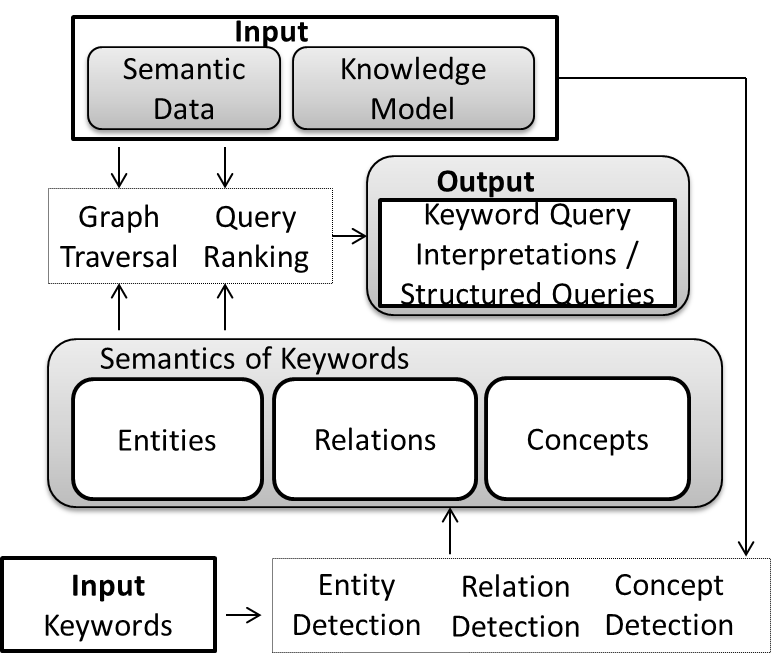
\includegraphics[width=0.34\textwidth]{figs/keywordinterpretation}}
  ~ %add desired spacing between images, e. g. ~, \quad, \qquad etc. (or a blank line to force the subfig onto a new line)
  \subfloat[Translating NL queries.]{\label{fig:inter_NL}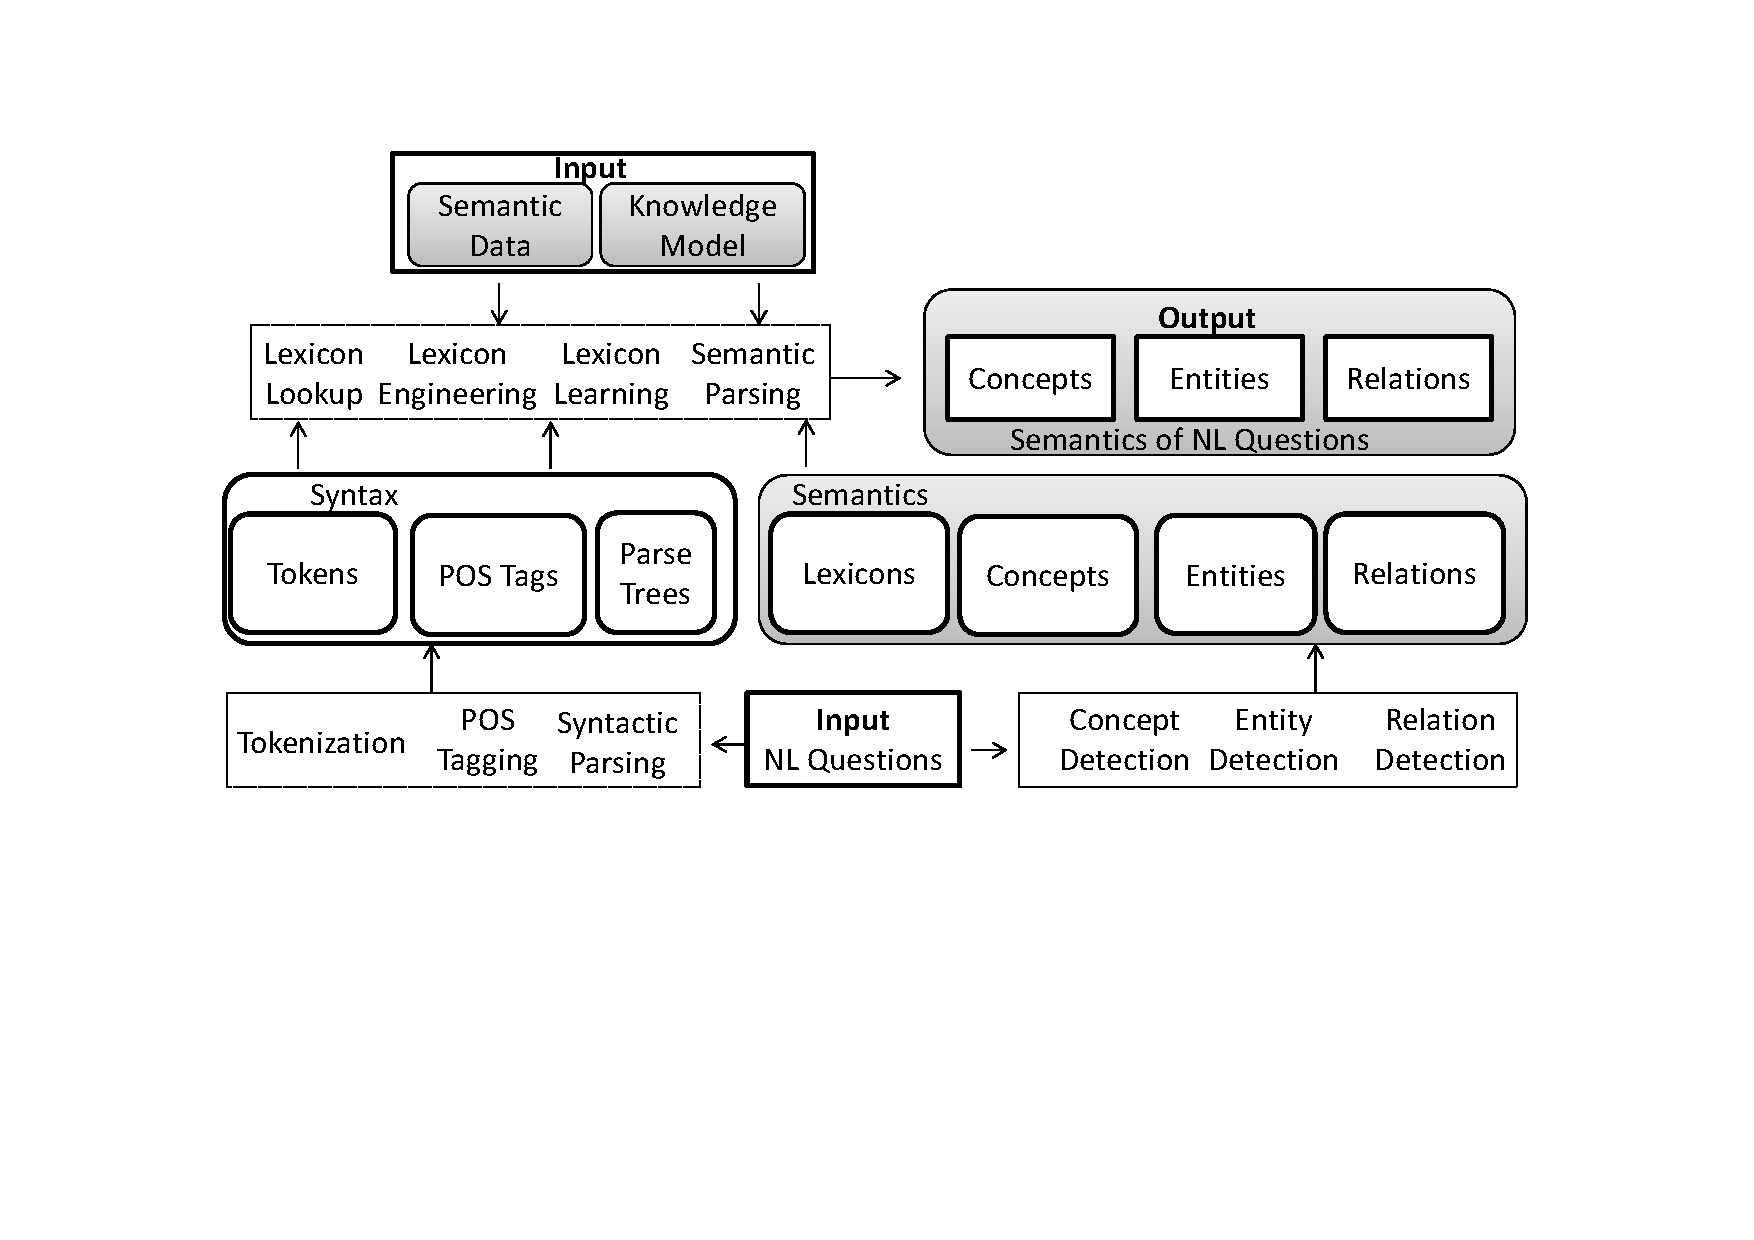
\includegraphics[width=0.6\textwidth]{figs/nlinterpretation}}
 \caption{Translating keywords and NL queries.}
 \label{fig:translation}
\end{figure*}


\subsection{Translating NL Queries} There are two main categories of approaches for dealing with this problem. One the one hand, it can be tackled in a way similar to the translation of keyword queries. This solution (depicted in the bottom left portion of Fig.~\ref{fig:inter_NL}) involves the detection of concepts, entities, and relations~\cite{DBLP:conf/aswc/CaoCT08}, and their mapping to elements of structured queries. The problem of ambiguity is solved here by using robust techniques for the matching of words in the NL query against elements in the semantic data and semantic models, and for the ranking and disambiguation of resulting matches. In fact, this kind of approaches is particularly popular among domain-independent NL query translation systems. AquaLog~\cite{DBLP:journals/ws/LopezUMP07}) for instance, maps words in NL queries to elements in the semantic data, and disambiguates results using domain-independent lexical resources (e.g. WordNet). 

As depicted in Fig.~\ref{fig:inter_NL}, the other category of approaches involves the use of lexicons, often in combination with a syntactic analysis tools. 
%Because NL questions also provide syntactic features, 
In fact, the same text analysis tools used for content interpretation can be applied here. For instance, the Stanford Parser~\footnote{\url{http://nlp.stanford.edu/software/lex-parser.shtml}} and GATE~\footnote{\url{http://gate.ac.uk/}} are used by FREyA~\cite{DBLP:conf/esws/DamljanovicAC10} to identify concepts in NL questions and to derive the syntactic parse tree, respectively. The use of domain-specific lexicons provide is a common way to deal with ambiguities, especially for traditional NL translation systems that are focused on a particular domain. Basically, a lexicon captures the mappings from syntactic elements to semantic elements. For instance, ORAKEL uses a lexicon, which specifies the mappings between nouns (verbs) with their arguments identified through the syntactic analysis and concepts (relations) in the semantic models~\cite{DBLP:journals/dke/CimianoHHMS08}. These mappings are specified by lexicon engineers. A different lexicon is needed when porting the NL interface from one domain to one other. Aiming at reducing this upfront customization effort and domain independence, there are also systems that in the case of lexical ambiguities, ask users to provide mappings, and use them to train models (e.g. via reinforcement learning~\cite{DBLP:conf/esws/DamljanovicAC10}) that automatically compute mappings. 

%Instead of performing the syntactic parsing separately from the mapping of syntactic elements to semantic elements, these two steps have been also  in one pass, called semantic parsing. 

%While it has been reported~\cite{DBLP:journals/ws/LopezUMP07} that domain customization usually improves recall, many NL-based semantic search systems exploit general domain-independent lexical resources (e.g. WordNet is used by AquaLog~\cite{DBLP:journals/ws/LopezUMP07}) but do not require domain-specific lexicons.

\subsection{Iterative Query Construction}

The discussed query interpretation approaches 
%deal with the interpretation of ambiguous queries that are expressed as NL or keywords. The 
aim at a more precise understanding of the information need, represented as a structured query. This is also the objective of other related approaches that fall into the general category of query construction. For instance, faceted search~\cite{DBLP:conf/dexa/WagnerLT11,DBLP:conf/esws/HeimEZ10,DBLP:conf/semweb/FerreH11} as well as the other kind of iterative query interfaces based on visual manipulation (drag and drop)~\cite{DBLP:journals/ws/Harth10} as presented before, also belong to this general category. In these systems, user operations are directly mapped to changes in the query. For instance, adding and removing facets result in the addition (query expansion) and removal (query refinement) of query predicates, respectively. Clearly, the difference to work on keyword and NL query interpretation is the lack of ambiguity, i.e. the semantics of every user input is clear. 
	
\section{Matching}\label{sec:matching}
% Table generated by Excel2LaTeX from sheet 'Tabelle1'
\begin{table}[htbp]
  \centering
  \caption{Overview of matching approaches.}
    \begin{tabular}{|c|c|c|}
    \hline
    \textbf{Term} & \textbf{Structure} & \textbf{Semantic} \bigstrut\\
    \hline
    \hline
    Syntactic-based & Join  & Forward chaining \bigstrut\\
    \hline
    Lexicon-based & Graph traversal & Backward chaining \bigstrut\\
    \hline
    \end{tabular}%
  \label{tab:addlabel}%
\end{table}%

\dtr{some systems may do interpretation, some not....}
The differences between term matching, structure matching and graph traversal are illustrated in Fig.~\ref{fig:matching}. 
	
\subsection{Term Matching} 
%\subsubsection{Term- / Content-based Matching}
This matching is needed when the representation of query and data is based on terms (i.e. is a bag of words). This is the case with all the existing concept-based document retrieval solutions~\cite{DBLP:conf/sigir/Giger88,DBLP:conf/sigir/ZhongH06,DBLP:conf/trec/JelierSEWMSMK03,DBLP:conf/sigir/QiuF93,DBLP:conf/sigir/QiuF93,DBLP:conf/sigir/Voorhees93,DBLP:conf/sigir/Voorhees94,DBLP:journals/ipm/MeijTRK10}, which identify the concepts behind the query and content but however, only use them for query or document expansion (i.e. expand the term-based query / content representation with additional terms corresponding to the identified concepts). Likewise, there are approaches, which interpret the query as entities and relations and to use this understanding to expand the queries with corresponding terms~\cite{DBLP:series/sci/NgoC10}. Many semantic data retrieval systems such as Falcons~\cite{DBLP:journals/ijswis/ChengQ09} and Sig.ma~\cite{DBLP:journals/ws/TummarelloCCDDD10} also employ bag-of-words representations -- both of the query and the semantic data. In these cases, the structure and semantics are not taken into account during the matching (but possibly, might have been used in other steps such as query interpretation). The matching boils down to the standard IR retrieval problem. Namely, given a set of keywords, documents matching individual keywords are retrieved. Typically, they are then joined to obtain those, which match all query keywords (AND-semantics). 
%This matching goes beyond the term-level to consider the content, which may contain several mentions of the query terms, as well as mentions of terms that do not appear in the query. At this content level, results may differ in the degree of matching, an aspect that is dealt with during the ranking. 

\subsection{Matching Complete Structure Patterns (Structure Matching)} 
	This matching is possible when the query and content are interpreted or are directly available as a structured query and semantic data, respectively. That is, the semantics of both the query and data is represented in terms of some entities and their relations. Most frequent is the combination SPARQL queries and RDF data. In particular, the three common types of information needs discussed previously can be captured through the basic graph pattern (BGP) feature of SPARQL. Just like semantic data, a BGP forms a graph where nodes and edges are either constants or variables. They form complete patterns in the sense that through explicitly captured join variables, the query engines know how to combine intermediate results obtained for subparts of the queries (for triple patterns in the BGP) to compute end results. Matching BGPs against semantic data boils down to the task of \emph{graph pattern matching} where constants in the BGP representing entities, relations, attributes and attribute values are matched against the RDF data graph to find matching subgraphs that contain bindings to variables in the BGP. Processing these BGPs involves standard \emph{database query evaluation} techniques, i.e. precompile the query to capture an optimal evaluation plan, then \emph{retrieve} data (from optimized indexes) for each triple pattern and \emph{join} intermediate results according to the plan. This matching is supported by off-the-shelf triple stores. For instance, it is used by SemSearchPro~\cite{DBLP:journals/ws/TranHL11} for computing results for SPARQL queries, after they have been derived from keywords through query interpretation. 
	
	\subsection{Matching Incomplete Structure Patterns (Graph Traversal)}  While join-based evaluation is possible for structured pattern that are complete, traversing the data graph is needed when query patterns entail missing connections. That is, the query engines cannot directly combine partial results based on join variables but needs to explore for different paths between them. One combination that involves this type of matching is the evaluation of keyword queries over semantic data. As discussed before, the structure and semantics in the data can be used to interpret the keyword query and to convert it to a structured query. Instead of query interpretation, there are also systems~\cite{DBLP:conf/cikm/LadwigT11,DBLP:conf/sigmod/LiOFWZ08}, which use the same \emph{graph traversal} mechanism to directly evaluate the keyword query. They skip the computation of queries and directly explore for results in the data (subgraphs) that match the keywords. As opposed to standard IR-style keyword search on documents, the results here are semantic data graphs. That is, the keywords in the query do not refer to single documents but possibly, several entities that are connected through paths in the semantic data graph. Hence, simply joining results (documents), which match the query keywords is not sufficient. Entities matching keyword(s) in the query have to be retrieved, and subgraphs containing paths, which connect these keyword matching entities have to be explored in the data through traversing graph nodes and edges. 
	
	A different semantics has been used~\cite{DBLP:conf/www/RochaSA04}, where results do not have to cover those nodes matching the query keywords. Those parts of the data, which are interesting and thus, shall be explored and returned as results, are controlled through manually defined traversal constraints that are realized via spreading activation. 

Interestingly, graph traversal is also employed for the relational search scenario, where the relations (paths) between entities are unknown. For instance, the mechanism used by for graph exploration by Hermes~\cite{DBLP:journals/ws/TranWH09,DBLP:conf/icde/TranWRC09}, a keyword search system, is similar to the one proposed for answering P-Queries~\cite{DBLP:conf/www/AnyanwuS03}, a special type of queries that ask for unknown semantic associations between entities. 

Another application of graph traversal has been proposed for the combined scenario of document and data retrieval. The goal is to find entities in the knowledge base, which are related to the documents to be retrieved, or vice versa, to retrieve documents related to some given entities. The starting points here are thus documents or entities, and traversal from these points are controlled through spreading activation~\cite{DBLP:conf/esws/SchumacherSS08}.


	\subsection{Reasoning} The formal well-defined semantics of some semantics models such as ontologies represented in OWL, have also be exploited for matching. More precisely, they are used for \emph{reasoning} to consider not only the available data but also new facts that can be automatically inferred from the formal semantics. For instance, the semantic models used in Serene~\cite{DBLP:journals/ws/FazzingaGGL11} is an ontology TBox represented as DL formulas, and semantic data are captured as ABox assertions of the same ontology. Serene uses an inference engine to derive new knowledge during an offline ontology compilation step. This computation is performed offline to improve the efficiency of online matching. Clearly, new knowledge relevant for the query can also be derived online. In ORAKEL for instance, the inference of new facts is performed as part of the computation of query matches. Notably, the first system created in the early years of Semantic Web research, which makes use of logical reasoning for computing semantic matches is SHOE~\cite{DBLP:conf/dagstuhl/HeflinHL03}. 
	
\subsection{Matching: Combination of Techniques}	
	
\section{Ranking}\label{sec:ranking}
Ranking approaches leverage different factors, which in general, can be \emph{query-independent} or \emph{query-dependent}. The latter considers the \emph{relevance} of the result with respect to the query. The former includes different aspects, such as \emph{rarity} (measured in terms of occurrence~\cite{DBLP:journals/internet/Aleman-MezaHARS05}), \emph{popularity} (based on occurrences~\cite{DBLP:conf/icde/TranWRC09}, or centrality~\cite{DBLP:journals/internet/Aleman-MezaHARS05}), \emph{predictability} (based on information content~\cite{DBLP:conf/www/AnyanwuMS05}), \emph{trust} (e.g. trust assigned to sources~\cite{DBLP:journals/internet/Aleman-MezaHARS05}) or \emph{confidence} (e.g. confidence scores of data extraction outputs~\cite{DBLP:conf/www/NieZWM05,DBLP:conf/vldb/ChengYC07}). They could be seen as heuristics, which can complement the ranking based on query-relevance. Among those heuristics, there are two prominent ones that are widely used in existing approaches, namely \emph{centrality-} and \emph{proximity-based ranking}. 

% Table generated by Excel2LaTeX from sheet 'Tabelle2'
\begin{table}[htbp]
  \centering
  \caption{Overview of centrality-based ranking.}
    \begin{tabular}{|p{3.5cm}|p{3.5cm}|}
    \hline
    Hyperlinks & Relations  \bigstrut\\
    \hline
    \hline
    Adoption of PageRank to (1) ontologies as documents, (2) two-layered graph with sources (documents) representing one layer & Authority transfer weights (1) specified by experts, (2) learned through simulated annealing or PARAFAC decomposition \bigstrut\\
    \hline
    \end{tabular}%
  \label{tab:addlabel}%
\end{table}%


\subsection{Centrality-based Ranking} The algorithms commonly used for computing centrality in the context of ranking is PageRank and HITS. Basically, the idea behind it is to perform link analysis on the graph formed by the hyperlink structure of documents to identify nodes that are important (or popular or authoritative). In the semantic search context, much effort has been invested in extending the original PageRank and HITS proposals towards dealing with semantic data graphs, where instead of documents and hyperlinks, there are entities that are connected through different types of semantic links. One of the first proposal for using PageRank for dealing with semantic data is OntoRank~\cite{DBLP:conf/semweb/DingPFJPK05}. However, ranking here is only dealt with at the level of sources, namely ontolgies (instead of the entities contained in them). PageRank could be directly applied because ontologies are treated as Web pages, and there are no different types of links. ObjectRank~\cite{DBLP:conf/vldb/BalminHP04} build upon PageRank, but recognizes the variety of semantic links. Instead of using the same authority flow for all edges, it employs an authority transfer schema graph, which captures the strengths of authority for different types of edges. While all these weights has to be manually specified by domain experts in ObjectRank, PopRank~\cite{DBLP:conf/www/NieZWM05} incorporates a simulated annealing algorithm to learn these weights, based on a partial weighting provided by experts. A different direction for obtaining the weights of semantic relations is taken by TripleRank, which models data by means of a 3-dimensional tensor. Applying the PARAFAC decomposition (a multi-modal counterpart to HITS) then results in authority and hub scores for both the entities and links. EntityAuthority~\cite{DBLP:conf/webdb/StoyanovichBBW07} operates not only on the semantic data graph but on a combined graph that contains both entities and documents as nodes. Also, a two-layer approach has been pursuit, where PageRank is computed both for the sources and the entities contained in them~\cite{DBLP:conf/esws/DelbruTCTD10,DBLP:conf/semweb/HarthKD09}. 

\subsection{Proximity-based Ranking} Another popular heuristic that has been successfully used in IR is the proximity between terms~\cite{DBLP:conf/sigir/ButtcherCL06a,DBLP:conf/sigir/TaoZ07}. According to this, a result is ranked high when it contains query terms that appear closer to each other in its textual content. 
Note that while it is not independent of the query, this heuristic does not directly capture the query-relevance. This notion of proximity has also been used for XML data retrieval: XRank proposes to rank results based on the smallest text window, which contains all matches to query keywords~\cite{DBLP:conf/sigmod/GuoSBS03}. The notion of proximity has also been adopted to the case of semantic data, where instead of textual proximity (distance between terms), the distance between semantic entities is taken into account. For document retrieval, several proximity measures have been proposed to measure the distance between named entities extracted from text~\cite{DBLP:conf/iiwas/LeCHC11}. In keyword search over semantic data, results are subgraphs containing nodes matching the query keywords. One of the factor often used for ranking these results is based on the (pair-wise) distances between keyword matching nodes (the length of the paths connecting them)~\cite{DBLP:conf/cikm/LadwigT11,DBLP:conf/icde/TranWRC09,DBLP:conf/sigmod/LiJLF09}. Similar to text proximity, the intuition here is that more compact results more likely correspond to the intended need. 

% Table generated by Excel2LaTeX from sheet 'Tabelle3'
\begin{table}[htbp]
  \centering
  \caption{Overview of query-relevance based ranking.}
    \begin{tabular}{|p{3.2cm}|p{3.8cm}|}
    \hline
    Content & Structure  \bigstrut\\
    \hline
    \hline
    Treat entities as documents and adopt (1) Vector Space Model (2) unstructured LM & (1) BM25F, (2) structured LM, (3) edge-specific relevance model, (4) triple-based LM \bigstrut\\
    \hline
    \end{tabular}%
  \label{tab:addlabel}%
\end{table}%


\subsection{Query-Relevance Based Ranking} Given the ambiguous query, different results can be found that vary in the degree relevance. This classic problem is extensively studied in IR. In the semantic search setting, existing IR concepts have been used and extended to deal with semantic data and to leverage the availability of semantics. 

Many semantic search systems, which provide keyword search over semantic data, apply standard IR ranking. For instance, Falcons~\cite{DBLP:journals/ijswis/ChengQ09} uses a standard IR tool (Lucene~\footnote{\url{http://lucene.apache.org/java/docs/index.html}}) to index entities as documents, and uses the built-in ranking mechanism for entity ranking.  

For ranking more complex (relational search) results, there are keyword search systems, which use the Vector Space Model and adopted the \emph{TFIDF-based} term weighting. The result in this setting is a graph, which contain a set of keyword matching nodes. A popular ranking is based on sum of the individual TF-IDF score computed for every keyword match via pivoted normalization weighting. Specific normalization methods have proposed to recognize that the textual length of the matching elements is often very short (document length normalization), different attributes can be associated with different vocabularies (IDF normalization) and a result is actually an �aggregation of documents� and thus requires additional normalization beyond the document level. Also TF-IDF has been adopted for the case of document retrieval using semantic data. Here the TF-IDF weighting has to be modified to consider not only the frequency of terms but also the frequency of named entities~\cite{DBLP:series/sci/NgoC10} and annotations~\cite{DBLP:journals/tkde/CastellsFV07}.  


Taking the specific semantics of entity results into account, an extension of the \emph{BM25F} has been proposed~\cite{DBLP:conf/semweb/BlancoMV11}. The idea is to use different fields for indexing different properties of RDF entities. Different weights are assigned to these fields to recognize that some properties are more important than others in ranking entities. 

Also, the more recent \emph{language modeling} (LM) paradigm has been adapted to this case of complex results. Language models for documents and queries are employed to represent them as multinomial distributions over words of the vocabulary. The KL-divergence, basically measuring the distance between the query and document distribution, can then be used for ranking. For ranking structured objects, three different models were studies~\cite{DBLP:conf/www/NieMSWM07}: The simple unstructured model treats all object attributes and values as vocabulary terms. The structured variant employs language models for specific components of the structured results. The record-level representation models an object through several language models, each capturing a record of that object. The attribute-level representation further segments a record into multiple fields and assigns different weights to individual fields (similar to the idea behind BM25F). Moreover, specific term distributions for fields have been proposed. Using edge-specific relevance models~\cite{DBLP:conf/cikm/BicerTN11}, the probability of observing a word in a structured result may vary, depending on the attribute (the edge) to be considered. This edge-specific model is employed not only to exploit the structure and semantics in the data but also to capture the semantics behind the keyword query. For this, an initial run over the semantic data is performed to obtain pseudo-relevance feedback (PRF) results for the keyword query. Instead of using the short and ambiguous keyword query, an edge-specific model constructed from these PRF results is used to capture the information need (the relevance). 

As opposed to the approaches mentioned before, which model queries and documents based on words, there are also language models defined as probability distributions over RDF triples~\cite{DBLP:journals/debu/ElbassuoniRSW10}. The probability of a given triple should capture its ``informativeness'', which is measured based on witness counts. The authors implement this by issuing keyword queries for each triple using Web search engines, and used the reported result sizes as witness count estimates. Following the same direction, NAGA~\cite{DBLP:conf/icde/KasneciSIRW08} not only uses informativeness but also a measure of confidence to estimate parameters of the language models. 

\subsection{Ranking: Combination of Factors}
Clearly, the ranking implemented by a system is often a combination of factors. For instance, for searching entities detected from documents, EntityRank~\cite{DBLP:conf/vldb/ChengYC07} rank entities based on the popularity of documents they have been extracted from (computed via PageRank), the confidence of the extraction outputs, contextual constraints as well as the proximity among entities and query words. For retrieving more complex objects (comprises multiple records) extracted from web documents, experiments with Libra (a scientific Web search engine) have shown that ranking can be improved when taking extraction confidences both at the record- and attribute-level into account~\cite{DBLP:conf/www/NieMSWM07}. Structured results (a subgraph) obtained from keyword search over structured data is mostly ranked based on the PageRank of its constituent nodes, aggregation of query-relevance scores obtained for individual nodes (records) matching query keywords, and the proximity defined through the length of paths between nodes~\cite{DBLP:conf/icde/TranWRC09}. 

\dtr{todo:learning to rank  \cite{DBLP:conf/cikm/CoffmanW11}}


\section{Main Approaches and Their Performances}\label{sec:approaches}	
Semantic search has been investigated from different communities in different context. In the IR community, semantic search has mainly been viewed from the perspective of \emph{document retrieval}. Here, classic \emph{conceptual} approaches based on the use of lexical models can be distinguished from more recent approaches that employ of \emph{annotations in the form of semantic data}. Another line of research is \emph{entity search}, which has been studied in the context of entities extracted from Web pages, Wikipedia pages corresponding to entities, and entities captured by databases and Semantic Web datasets. Another popular topic is \emph{keyword search over databases and Semantic Web data}, which is mainly about relational information. Last but not least, the \emph{processing of NL questions} entail specific challenges and opportunities, which has attracted attention from a specific community of researchers. We will now discuss the role of semantics in solving these different search tasks and its impact on performance. 

\subsection{Conceptual Document Retrieval} This is the classic type of semantic search systems, which has been studied already in the early years of IR research. Researchers have recognized for a richer representation of the information needs and data that goes beyond the bag-of-words model. It became evident that constructing a full-fledge logic-based representation~\cite{DBLP:conf/sigir/Rijsbergen89} for queries and especially for documents is not practical. Thus, lightweight \emph{lexical models} have been employed to interpret the semantics of query and documents as concepts, and used within standard bag-of-words IR paradigm (e.g. vector space model and language model). Then, retrieval may be done based on concepts alone, or in the form of query and document expansion. In the latter case, bag-of-words model constitutes the basis while the conceptual understanding helps to refine or add more relevant words. However, there are \emph{no clear evidences suggesting conceptual IR can outperform standard IR techniques}. It has been shown that automatic query expansion in the large diverse TREC collection using WordNet degrades performance. Even when selected by hand, it helps only when the query is an incomplete description of the need~\cite{DBLP:conf/sigir/Voorhees94}. More recently, it has been shown for the medical domain (TREC Genomics) that retrieval based on concepts alone could not outperform the standard baseline based on words~\cite{DBLP:conf/trec/TrieschniggKS06,DBLP:conf/trec/ZhouYTS06}. Current work in this direction, which combines concepts and bag-of-words in the form of query expansion, outperforms a state of the art baseline in one collection, and shows similar performances in other collections~\cite{DBLP:journals/ipm/MeijTRK10}. However, the experiments have been performed on 
collections where documents have been manually annotated with concepts (domain-specific CLEF and TREC Genomics collections). 


\subsection{Annotation-based Document Retrieval} This encompasses the newer type of approaches, which exploit advancements in data extraction technologies to obtain a richer representation of queries and documents, namely as entities and relations represented as annotations (query and document annotations, respectively). To date, there exist only anecdotal evidences for the merits of this type of systems. Possibly, the most conclusive result in this direction is based on experiments using the TREC Question Answering track: For a subset of manually chosen questions, it has been shown that higher precision could be obtained~\cite{DBLP:conf/sigir/Chu-CarrollPCFD06}. The results there can also be interpreted as follows: The employed data extraction programs were optimized for a few specific types of relations and entities (e.g. \verb+Person+). High precision is possible for questions that can be covered by these types of annotations. However, high recall is difficult because it requires the data extraction program to recognize arbitrary types of entities and relations. While there are promising ideas towards this kind of open data extraction, this problem remains an open challenge. Along this line, there is a study showing that the quality of data extractions significantly impacts search performance~\cite{DBLP:conf/cikm/Chu-CarrollP07}. 


\subsection{Entity Search} While the two mentioned types focus on documents, this category includes search over (1) documents (for processing factoid and list questions of the TREC QA track~\cite{DBLP:conf/sigir/Chu-CarrollPCFD06}, or for expert search questions of the TREC Enterprise track~\cite{DBLP:journals/ipm/BalogAR09}), over Wikipedia data, which as discussed, can be seen as a kind of semantic data, or (2) documents associated with metadata, (for answering entity related questions of the INEX Entity Ranking track~\cite{DBLP:conf/cikm/KapteinSVK10,DBLP:conf/ecir/PehcevskiVT08}), or over pure (3) semantic data (for answering entity queries of the SemSearch Entity track~\cite{DBLP:conf/semweb/BlancoMV11}). Some type(1) systems can also be categorized as annotation-based document retrieval systems because they detect entities and relations in data and queries~\cite{DBLP:conf/vldb/ChengYC07,DBLP:conf/www/NieMSWM07,DBLP:conf/sigir/Chu-CarrollPCFD06}. As discussed, it has been shown that precision can be improved when high quality extraction outputs are available~\cite{DBLP:conf/sigir/Chu-CarrollPCFD06}. The use of semantics in type(2) systems is limited to viewing Wikipedia pages as entities~\cite{DBLP:conf/cikm/KapteinSVK10}, exploiting categories associated with them~\cite{DBLP:journals/tois/BalogBR11} and links between them~\cite{DBLP:conf/ecir/PehcevskiVT08}. It has been shown that Wikipedia articles can be effectively used as a pivot for entity search on the Web: it contain entities for a large amount of queries as well as cues (e.g. external links) that can be used to effectively find entities' official homepages on the Web~\cite{DBLP:conf/cikm/KapteinSVK10}. As a source of semantics, experiments have shown that category information helps to interpret the query and entity documents and to outperform standard text-based retrieval~\cite{DBLP:conf/cikm/KapteinSVK10,DBLP:journals/tois/BalogBR11}. While many type(3) systems~\cite{DBLP:journals/ijswis/ChengQ09,DBLP:journals/ws/HoganHUKPD11,DBLP:journals/ws/TummarelloCCDDD10,DBLP:journals/ws/TranWH09} have been built to search for entities over data crawled from the Semantic Web, solutions for ranking and the evaluation of their results have attracted interest only recently. The best performed method~\cite{DBLP:conf/semweb/BlancoMV11} is based on BM25F, which ranks entities as documents that are segmented into different fields corresponding to entity attributes. 

 

\subsection{Relational Keyword Search}
This category comprises all approaches, which process keyword queries over semantic data~\cite{DBLP:conf/icde/TranWRC09,DBLP:conf/cikm/LadwigT11,DBLP:conf/sigmod/LiOFWZ08}. While the results here include entities, the focus is to find possibly complex subgraphs encompassing several entities and relations between them (i.e. to support relational search). There exist a variety of indexing strategies and traversal algorithms that help to perform this task more efficiently. However, recent work~\cite{DBLP:conf/cikm/CoffmanW10} has shown that the proposed ranking strategies~\ref{DBLP:conf/icde/TranWRC09,DBLP:conf/sigmod/LiuYMC06} based on the adoption of proximity, TFIDF and PageRank do not perform well when considering a broad range of queries. This work aims at a standardized framework and benchmark for evaluating the effectiveness of relational keyword search approaches~\cite{DBLP:conf/cikm/CoffmanW10}. Based on this benchmark, it has been shown that best performance can be achieved through the use of edge-specific language models that are constructed for results and queries (based on PRF results)~\cite{DBLP:conf/cikm/BicerTN11}. \dtr{compare to recent learning to rank approach \cite{DBLP:conf/cikm/CoffmanW11}}. 

\subsection{NL Question Answering} \dtr{are there benchmarks for NL QA over data?}


% Table generated by Excel2LaTeX from sheet 'Tabelle1'
\begin{table*}[htbp]
  \centering
  \caption{Add caption}
    \begin{tabular}{r|r|r|r|r|r|r|r|r|r}
    \hline
          &       & C-Search & IBM   & Falcons & Yahoo! & AquaLog & Hermes & Naga  & TASTIER \bigstrut\\
    \hline
    \multicolumn{1}{l|}{\multirow{3}[6]{*}{Need}} & \multicolumn{1}{l|}{Entity} &       &       &       &       &       &       &       &  \bigstrut\\
\cline{2-10}    \multicolumn{1}{l|}{} & \multicolumn{1}{l|}{Fact} &       &       &       &       &       &       &       &  \bigstrut\\
\cline{2-10}    \multicolumn{1}{l|}{} & \multicolumn{1}{l|}{Relation} &       &       &       &       &       &       &       &  \bigstrut\\
    \hline
    \multicolumn{1}{l|}{\multirow{4}[8]{*}{Query}} & \multicolumn{1}{l|}{Keyword} &       &       &       &       &       &       &       &  \bigstrut\\
\cline{2-10}    \multicolumn{1}{l|}{} & \multicolumn{1}{l|}{NL} &       &       &       &       &       &       &       &  \bigstrut\\
\cline{2-10}    \multicolumn{1}{l|}{} & \multicolumn{1}{l|}{Facet} &       &       &       &       &       &       &       &  \bigstrut\\
\cline{2-10}    \multicolumn{1}{l|}{} & \multicolumn{1}{l|}{Iterative} &       &       &       &       &       &       &       &  \bigstrut\\
    \hline
    \multicolumn{1}{l|}{\multirow{3}[6]{*}{Data}} & \multicolumn{1}{l|}{Raw Data} &       &       &       &       &       &       &       &  \bigstrut\\
\cline{2-10}    \multicolumn{1}{l|}{} & \multicolumn{1}{l|}{Semantic Data} &       &       &       &       &       &       &       &  \bigstrut\\
\cline{2-10}    \multicolumn{1}{l|}{} & \multicolumn{1}{l|}{Semantic Metadata} &       &       &       &       &       &       &       &  \bigstrut\\
    \hline
    \multicolumn{1}{l|}{\multirow{2}[4]{*}{Semantic Model}} & \multicolumn{1}{l|}{Lexical} &       &       &       &       &       &       &       &  \bigstrut\\
\cline{2-10}    \multicolumn{1}{l|}{} & \multicolumn{1}{l|}{Knowledge} &       &       &       &       &       &       &       &  \bigstrut\\
    \hline
    \multicolumn{1}{l|}{\multirow{3}[6]{*}{Interpretation}} & \multicolumn{1}{l|}{Concept} &       &       &       &       &       &       &       &  \bigstrut\\
\cline{2-10}    \multicolumn{1}{l|}{} & \multicolumn{1}{l|}{Entity} &       &       &       &       &       &       &       &  \bigstrut\\
\cline{2-10}    \multicolumn{1}{l|}{} & \multicolumn{1}{l|}{Relation} &       &       &       &       &       &       &       &  \bigstrut\\
    \hline
    \multicolumn{1}{l|}{\multirow{4}[8]{*}{Matching}} & \multicolumn{1}{l|}{Term } &       &       &       &       &       &       &       &  \bigstrut\\
\cline{2-10}    \multicolumn{1}{l|}{} & \multicolumn{1}{l|}{Structured Pattern } &       &       &       &       &       &       &       &  \bigstrut\\
\cline{2-10}    \multicolumn{1}{l|}{} & \multicolumn{1}{l|}{Reasoning} &       &       &       &       &       &       &       &  \bigstrut\\
\cline{2-10}    \multicolumn{1}{l|}{} & \multicolumn{1}{l|}{Traversal} &       &       &       &       &       &       &       &  \bigstrut\\
    \hline
    \multicolumn{1}{l|}{\multirow{3}[6]{*}{Ranking}} & \multicolumn{1}{l|}{Centrality} &       &       &       &       &       &       &       &  \bigstrut\\
\cline{2-10}    \multicolumn{1}{l|}{} & \multicolumn{1}{l|}{Proximity} &       &       &       &       &       &       &       &  \bigstrut\\
\cline{2-10}    \multicolumn{1}{l|}{} & \multicolumn{1}{l|}{Query Relevance} &       &       &       &       &       &       &       &  \bigstrut\\
    \hline
    \end{tabular}%
  \label{tab:addlabel}%
\end{table*}%



%\section{Semantic Data Retrieval}
\subsection{Applications} 
\subsection{Semantic Data Retrieval Process} 
- Crawling, integration, indexing, matching \& ranking, result presentation \\

\subsection{Taxonomy of Semantic Data Retrieval Approaches}
- overview of existing approaches categorized along the dimensions: need, data, queries, targeted task in the process \\
- following survey focus on keyword queries  \\


\subsection{Semantic Data Crawling} 
\subsection{Semantic Data Integration}
\subsection{Semantic Data Storage and Indexing}
\subsection{Semantic Search Result Presentation}

 

%\section{Matching \& Ranking in Semantic Data Retrieval}

\subsection{Query-Independent Ranking}
- Existing approaches based on PageRank

\subsection{Term-based Matching \& Ranking}
- Does not consider structure information \\
- Most existing engines use simple TF/IDF term weighting, do not take structure information into account 

\subsection{Term-based Matching \& Structured-based Ranking}
- Take structure of data \& results into account for ranking\\
-	BM25F\\
- Language model for structured results

\subsection{Term- and Structure-based Matching \& Ranking} 
-	Matching: take structure of data account for computing structured results

\section{Open Research Challenges}\label{sec:challenges}




\bibliographystyle{elsart-num-sort}

\bibliography{paper}

\clearpage

\end{document}
